%!TEX root = ../thesis.tex

\chapter{Background}\label{ch:background}
We begin this thesis by introducing the required technical back, most notably defining the flow map of a deterministic system and building up to It\^o stochastic differential equations as a means of incorporating uncertainty into these models.
Further details on the technical results and tools employed later are provided in \Cref{app:theory}.
The chapter is concluded by summarising stochastic sensitivity \citep{Balasuriya_2020_StochasticSensitivityComputable}, which provided initial tools for characterising uncertainty in a computationally efficient manner and was the primary motivation for this work.

% In this chapter, we first motivate the need for stochastic models with a simple example predicting the path of a drifter in the Gulf Stream.o

% Throughout, we will use an example of tracking a drifter in the Gulf Stream to illustrate the concepts introduced.
% We will return to this example in more detail, including applying our later developments, in \Cref{ch:appls}.

% We then briefly review the current literature on stochastic parameterisation, which is the introduction of stochastic terms into otherwise deterministic models, in the context of atmospheric modelling, oceanography and climate forecasting.
% Finally, we highlight the limitations of bulk stochastic simulation as a means of working with complicated stochastic models, both in terms of computational costs and accuracy.
% This suggests the need, across a variety of applications, for developing computationally efficient methods for approximating prediction distributions of such stochastic models, which this thesis aims to address.


\section{Notation}
We adopt several notational conventions throughout this thesis, which are summarised here.
The set of \(n \times m\) matrices with real-valued entries is denoted as \(\R^{n\times m}\).
% In general, the \(i\)th component of a vector \(x\) is denoted by \(x_{i}\), except where there is already a subscript, in which case we write \(x_t^{(i)}\) to denote the \(i\)th component of \(x_t\), for instance.
% For a matrix \(A\), \(\left[A\right]_{\cdot i}\) typically refers to the \(i\)th column, and \(\left[A\right]_{i\cdot}\) the \(i\) the row of \(A\).
The norm symbol \(\norm{\cdot}\) without any additional qualifiers denotes the standard Euclidean norm for a vector, and the spectral (operator) norm induced by the Euclidean norm, i.e.\ for an \(n \times n\) matrix \(A\)
\[
	\norm{A} = \sup\left\{\frac{\norm{Av}}{\norm{v}}\,\middle|\,v \in \R^n, \, \norm{v} \neq 0\right\}.
\]
For a random variable \(X\), we use \(\avg{X}\) to denote the expectation of \(X\) and \(\var{X}\) to denote the variance.
For a \(n\)-dimensional vector-valued random variable \(Y\), \(\avg{Y}\) again denotes the (now vector-valued) expectation of \(Y\), and \(\var{Y}\) denotes the covariance matrix of \(Y\).
That is, \(\var{Y}\) is the symmetric \(n\times n\) matrix with \((i,j)\)th component
\[
	\left[\var{Y}\right]_{ij} = \avg{Y_iY_j} - \avg{Y_i}\avg{Y_j} = \cov{Y_i, Y_j} = \begin{cases}
		\var{Y_i},      & \text{if } i = j, \\
		\cov{Y_i, Y_j}, & \text{otherwise},
	\end{cases}
\]
where
\[
	\cov{Y_i, Y_j} = \avg{\left(Y_i - \avg{Y_i}\right)\left(Y_j - \avg{Y_j}\right)}
\]
denotes the (scalar) covariance between \(Y_i\) and \(Y_j\).

\begin{figure}
	\begin{center}
		\begin{tikzpicture}
			\node (as) [draw] {Convergence almost surely};
			\node (p) [draw, below=of as] {Convergence in probability};
			\node (rm) [draw, right=of p] {Convergence in \(r\)th mean, \(r > 0\)};
			\node (qm) [draw, above=of rm] {Convergence in \(q\)th mean, \(q > r\)};
			% \node (rmom) [draw, below=of rm] {Convergence of \(r\)th moment};
			\node (d) [draw, below=of p] {Convergence in distribution};
			\path[->,thick] (as) edge  (p)
			(p) edge  (d)
			(qm) edge (rm)
			(rm) edge (p);
			% (rm) edge (rmom);
		\end{tikzpicture}
		\caption{The strength of each notion of convergence for random variables, where each directed arrow corresponds to an implication.
			These results are stated and proven in \citet{Bremaud_2020_ProbabilityTheoryStochastic}, for instance.}
		\label{fig:rv_conv_impl}
	\end{center}
\end{figure}

There are several different notions of convergence for a sequence of random variables, which we briefly recall here.
Consider a sequence of \(m\)-dimensional random vectors \(X_1, X_2,\dotsc\) and an \(m\)-dimensional random vector \(X\).
We say that:
\begin{itemize}
	\item The sequence \(X_1, X_2, \dotsc\) converges \emph{in distribution} to \(X\) if
	      \[
		      \lim_{n\to\infty}F_n\left(x\right) = F(x),
	      \]
	      where \(F_n\) is the cumulative distribution function for \(X_n\) and \(F\) is the cumulative distribution function for \(X\), for every point \(x \in \R^m\) where \(F\) is continuous.
	      If this is the case, we write
	      \[
		      X_n \xlongrightarrow[\text{distribution}]{} X, \quad \text{as } n \to \infty.
	      \]
	      Note that the limiting random vector \(X\) need not be defined on the same probability space as the terms in the sequence \(X_1, X_2, \dotsc\); convergence in distribution is the only notion of convergence for which this is the case.


	\item The sequence \(X_1, X_2, \dotsc\) converges \emph{in probability} to \(X\) if for every \(\delta > 0\)
	      \[
		      \lim_{n\to\infty}P\left(\norm{X_n - X} < \delta\right) = 0,
	      \]
	      in which case we write
	      \[
		      X_n \xlongrightarrow[\text{probability}]{} X, \quad \text{as } n \to \infty.
	      \]

	\item The sequence \(X_1, X_2, \dotsc\) converges \emph{almost surely} to \(X\) if
	      \[
		      P\left(\lim_{n \to \infty}X_n = X\right) = 1,
	      \]
	      in which case we write
	      \[
		      X_n \xlongrightarrow[\text{almost surely}]{} X, \quad \text{as } n \to \infty.
	      \]

	\item For \(r > 0\), the sequence \(X_1, X_2, \dotsc\) converges \emph{in \(r\)th mean} to \(X\) if
	      \[
		      \lim_{n\to\infty}{\avg{\norm{X_n - X}^r}} = 0,
	      \]
	      in which case we write
	      \[
		      X_n \xlongrightarrow[r\text{th mean}]{} X, \quad \text{as } n \to \infty.
	      \]
	      This type of convergence is also known as \emph{\(L_r\)-convergence}, as it corresponds to convergence in the \(L_r\) norm on the probability space on which \(X_1,\dotsc, X_n\) and \(X\) are defined.

\end{itemize}
There are implications between each notion of convergence, with convergence almost surely being the strongest and convergence in distribution the weakest.
These implications are summarised in \Cref{fig:rv_conv_impl}.

We often work with stochastic processes that evolve through time, for example the Wiener process or the solution to a stochastic differential equation.
We generically use the notation \(y_t\), for instance, to denote the stochastic process, where \(t\) refers to time and \(y\) is a label.
The index set of the process is always a finite time interval, typically initialised at \(0\).
In almost all cases where we are working with \(y_t\) mathematically, \(y_t\) refers to the state of the process at the \emph{fixed} time \(t\).
When discussing a stochastic process in our prose, we also use \(y_t\) to refer to the \emph{full} solution path (where the range of \(t\) is known in context); this is an abuse of notation, but has no impact on the rigour of our mathematical results.




\section{The flow map}
Ordinary differential equations are used to model many different phenomena across a range of fields and applications.
Specifically, the continuous time evolution of a multi-dimensional state variable is governed by a system of first order differential equations of the form
\begin{equation}\label{eqn:det_ode}
	\dod{w_t}{t} = u\!\left(w_t, t\right),
\end{equation}
where \(w_t \in \R^n\) is the time-evolving variable of interest and \(u\) is the vector field specified at each relevant state and time \(t\).
The vector field \(u\) may be derived from a specified model, or may be driven or supplemented by observed data.
Since data has a finite-time limitation, we typically consider the evolution of \cref{eqn:det_ode} over a finite time interval \([0,T]\).
% In this thesis, we restrict ourselves to the finite time setting.
We can solve \cref{eqn:ode_det} analytically, or, as is often required in practice, numerically to generate time evolving trajectories, which can inform future predictions or be used to reconstruct past behaviour.
% The solutions to the differential equations of the form \cref{eqn:det_ode} define a continuous-time dynamical system.
The flow map of \cref{eqn:det_ode} provides a convenient way of summarising the trajectories that solve \cref{eqn:det_ode} and working with these solutions analytically.
Formally, the flow map \(F_{s}^{t}: \R^n \to \R^n\) from time \(s\) to \(t\) associated with \cref{eqn:det_ode} is the unique solution to
\begin{equation}
	\dpd{F_{s}^{\tau}\!\left(x\right)}{\tau} = u\left(F_{s}^\tau\!\left(x\right), \tau\right), \qquad F_{s}^{s}\!\left(x\right) = x,
	\label{eqn:flow_map_ode}
\end{equation}
solved up to time \(\tau = t\).
That is, the flow map is the operator mapping initial conditions at time \(t\) to their corresponding positions at time \(s\), under the continuous-time evolution of \cref{eqn:det_ode}.
Equivalently, the flow map satisfies the integral form of \cref{eqn:det_ode}:
\begin{equation*}
	F_s^t\!\left(x\right) = x + \int_s^t{u\!\left(F_s^{\tau}\!\left(x\right), \tau\right)\dif \tau}.
\end{equation*}
We use the flow map to represent all solutions of the deterministic differential equation \cref{eqn:det_ode}, with the understanding that for any relevant initial condition, the flow map at that point can be readily computed by solving the ODE either analytically or numerically.
For a well-defined flow, the flow map \(F_s^t\) is reversible, in that we could have \(t < s\), with the property
\[
	F_s^t\!\left(F_t^s\!\left(x\right)\right) = x,
\]
for any times \(s\) and \(t\).
We view the flow map primarily as a function of the initial condition, so that it quantifies the impact of changes in the initial condition on future predictions.
Accordingly, the gradient \(\nabla F_s^t\) of the flow map (with respect to the initial condition) provides insight into the local behaviour of the dynamical system \citep{Arnold_1973_OrdinaryDifferentialEquations,TruesdellNoll_2004_NonLinearFieldTheories}.
For any times \(s, t \in [0,T]\), this gradient	\(\nabla F_s^t\) satisfies a useful property:
\begin{equation}
	\dpd{\nabla F_{s}^{t}\!\left(x\right)}{t} = \nabla u\!\left(F_{s}^{t}\!\left(x\right), t\right) \nabla F_{s}^{t}\!\left(x\right),
	\label{eqn:eqn_of_variations}
\end{equation}
which is the equation of variations corresponding to \cref{eqn:det_ode}.
This result can be shown by taking the gradient of both sides in \cref{eqn:flow_map_ode} and using the chain rule.




\section{From ODEs to SDEs}
Differential equations are well-studied and ubiquitously employed across many fields.
These models are \emph{deterministic}, in that given an initial condition an ODE provides a single prediction of the future state.
However, as discussed in the introduction, in practice any such model will be subject to unavoidable uncertainty which can arise from a range of sources.
By accounting for any of these in our model, we expect to improve the power and accuracy of our predictions.
However, the true nature of this uncertainty is unknowable, so it is common to model it as a random process.
That is, we extend our deterministic model to a \emph{stochastic} one, where the solution (and therefore our predictions of the future state) is now a random variable with a probability distribution defined over the state space.
There are several approaches to establishing such a framework, the most general of which is a random dynamical system \citep{Arnold_1998_RandomDynamicalSystems,NeckelRupp_2013_RandomDifferentialEquations}.
When working in a continuous-time and continuous-state modelling scenario, a natural extension of an ordinary differential equation to account for this uncertainty is a stochastic differential equation (SDE) \citep{Oksendal_2003_StochasticDifferentialEquations,KallianpurSundar_2014_StochasticAnalysisDiffusion}, where the uncertainty is modelled with an additional term.
Although an SDE is an ``improvement'' over the deterministic ODE, in the sense that uncertainty can be encoded in the model itself, the compromise is that solutions are no longer straightforward to obtain or even analyse.
In fact, the formal treatment of SDEs requires an entirely new notion of integration, as we shall discuss.
Nonetheless, SDEs provide a rich framework for modelling and are used as predictive tools in a range of applications and fields. % \citep{Balasuriya_2020_StochasticApproachesLagrangian,SarkkaSolin_2019_AppliedStochasticDifferential,Oksendal_2003_StochasticDifferentialEquations,Jazwinski_2014_StochasticProcessesFiltering}.
There are several different ways to construct stochastic differential equations from deterministic dynamics; the following motivation of stochastic differential equations loosely follows a similar one available in \citet{Oksendal_2003_StochasticDifferentialEquations}, but other formulations of SDEs are available, e.g.\ using rough path theory \citep{FrizVictoir_2010_MultidimensionalStochasticProcesses} or by averaging the `fast' dynamics in a multiscale system \citep{MelbourneStuart_2011_NoteDiffusionLimits,GottwaldMelbourne_2013_HomogenizationDeterministicMaps,PavliotisStuart_2008_MultiscaleMethods}.

Suppose that we have a deterministic ordinary differential equation, i.e.\ \cref{eqn:ode_det}, and aim to account for uncertainty in the vector field \(u\).
In lieu of any additional understanding of this uncertainty, we model it as a stochastic noise.
Ideally, we would parameterise the uncertainty with some continuous-time stochastic process \(\xi_t\), and write
\begin{equation}\label{eqn:fake_sde}
	\dod{y_t}{t} = u\left(x_t, t\right) + \sigma\!\left(x_t, t\right)\xi_t,
\end{equation}
where \(\sigma\) is a specified part of the model that modulates how the magnitude and structure of the uncertainty varies with state and time.
Since we are modelling with a continuum, the noise process \(\xi_t\) should be (with probability \(1\)) continuous in time, and should, without any additional prior knowledge, evolve independently of itself through time, follow a probability distribution that does not depend on time, and have zero expectation.
That is, \(xi_t\) should be a white noise process in the absence of any additional knowledge of the nature of the noise, beyond the specification of \(\sigma\).
However, there does not exist \emph{any} process \(x_t\) that satisfies all of these properties \citep{Oksendal_2003_StochasticDifferentialEquations}; continuity cannot be enforced.
This complication requires an alternative formulation, which leads to an entirely new type of calculus built around the It\^o integral and It\^o stochastic differential equations, which we introduce in \Cref{sec:bkg_ito} and \Cref{sec:bkg_sde} respectively.

% In most modelling situations, we expect that the noise process \(\xi_t\) should have the properties:
% \begin{enumerate}
% 	\item For any two distinct times \(s \neq t\), the random variables \(\xi_s\) and \(\xi_t\) are independent.
% 	\item The process is stationary, that is the joint distribution of \(\xi_{t_1 + t}, \dotsc, \xi_{t_k + t}\) does not depend on \(t\).
% 	\item For all \(t\), \(\avg{\xi_t} = 0\).
% \end{enumerate}
% Additionally, since we are modelling with a continuum, the noise process \(\xi_t\) should be (with probability \(1\)) continuous in time.
% However, such a noise process \(\xi_t\) does not exist \citep{Oksendal_2003_StochasticDifferentialEquations}, in that there is no  continuous process with properties 1 to 3, so we need an alternative formulation of the integral.
% This leads to the It\^o integral, and It\^o stochastic differential equations, which we introduce in \Cref{sec:bkg_ito} and \Cref{sec:bkg_sde} respectively.

\subsection{The Wiener process}

\begin{figure}
	\begin{center}
		% 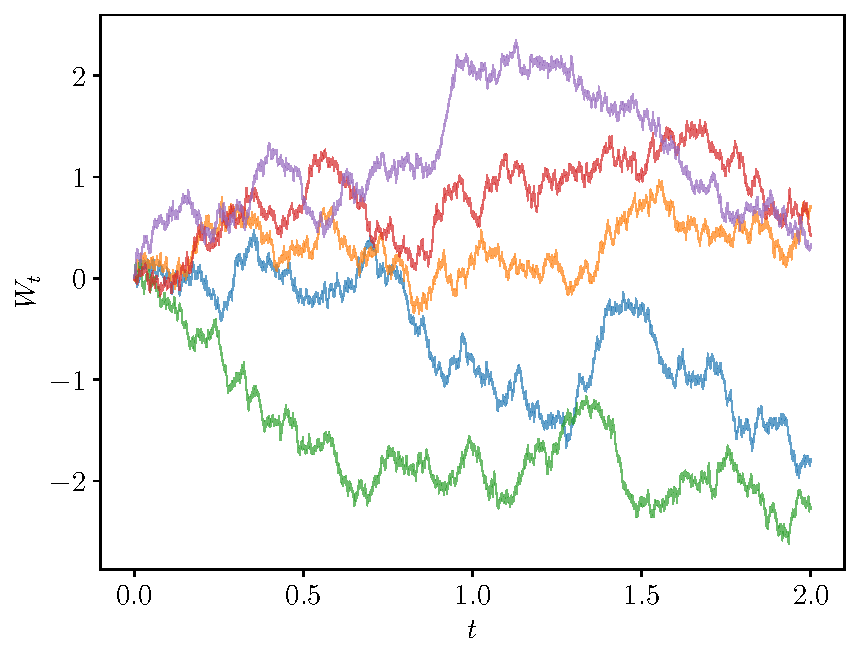
\includegraphics[width=0.49\textwidth]{chp02_background/figures/wiener_realisations_1d.pdf}
		% 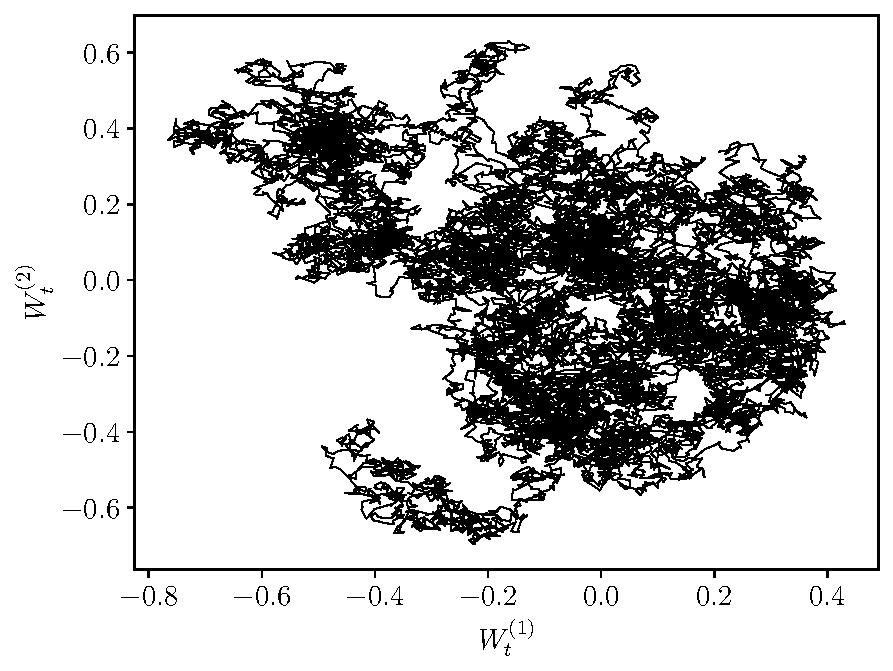
\includegraphics[width=0.49\textwidth]{chp02_background/figures/wiener_realisations_2d.pdf}
		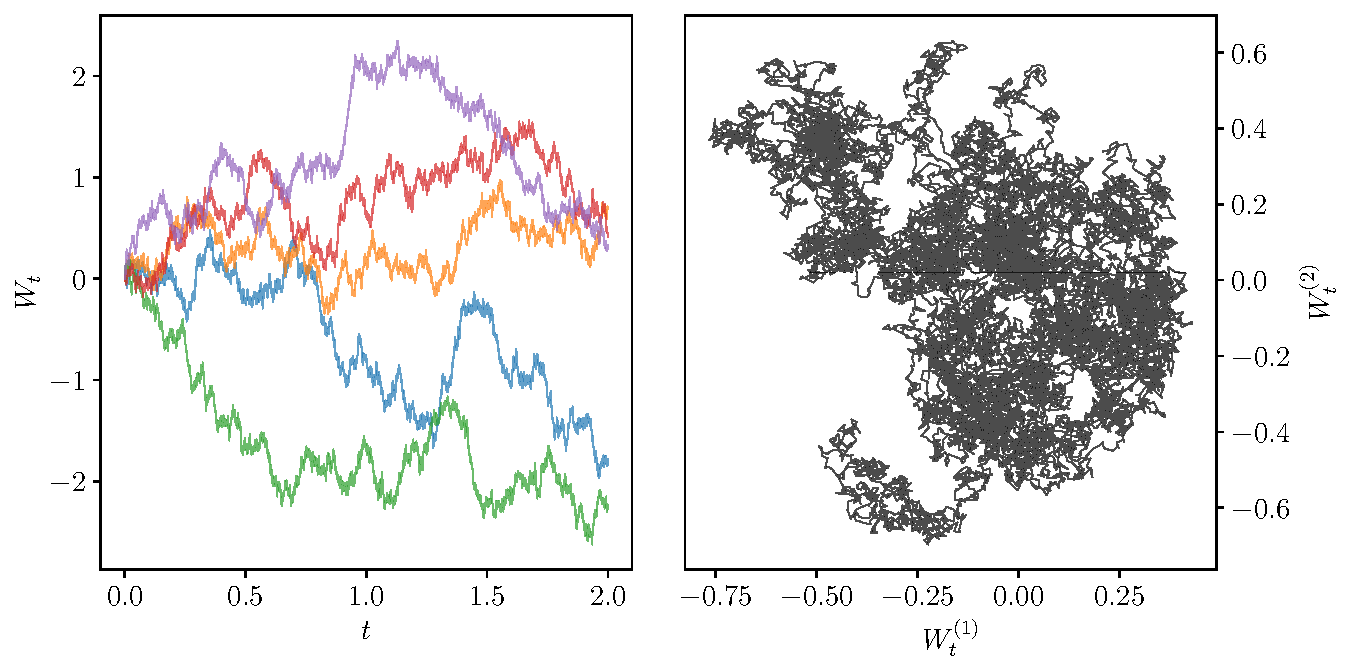
\includegraphics[width=\textwidth]{chp02_background/figures/wiener_realisations}
		\caption{(Left) Several realisations of a 1-dimensional Wiener process \(W_t\) evolving through time, and (right) a realisation of 2-dimensional Wiener process \(\left(W_t^{(1)}, W_t^{(2)}\right)^{\T}\).}
		\label{fig:wiener_rels}
	\end{center}
\end{figure}

In the absence of any additional knowledge about the nature of the noise (such as skew), the canonical Wiener process is the standard choice as the driving stochastic process.
The Wiener process is the definite integral of a white noise process, and is therefore an appropriate choice to ensure that the ``solution'' (the result after integration through time) of \cref{eqn:fake_sde} involves the idealised noise process \(\xi_t\) that we were initially after. %\lb{I don't think this makes any sense to the reader, but it's difficult to explain this intuitively. I believe that the idea is that this white noise process is the `derivative' of the Wiener process (in the sense that \(W_t\) is the integral of \(\xi_t\)).}.
Defined formally, the (1-dimensional) canonical \emph{Wiener process} is a stochastic process \(B_t\) taking values in \(\R\) and satisfying the following properties \citep{KallianpurSundar_2014_StochasticAnalysisDiffusion}:
\begin{romanate}
	\item \(B_0 = 0\) almost surely,
	\item for every \(s > 0\), the increments \(B_{s + t} - B_{s}\) for \(t \geq 0\) are independent of \(B_r\) for all \(r < s\),
	\item \(B_{s + t} - B_t \isGauss{0, s}\) for all \(s,t > 0\), and
	\item \(B_t\) is continuous in \(t\) almost surely.
\end{romanate}
Remarkably, these properties \emph{uniquely} define the Wiener process, with the additional result that for any \(t > 0\), \(B_t\) is distributed as \(\mathcal{N}\left(0, t\right)\), a Gaussian distribution with mean zero and variance \(t\).
The \emph{\(n\)-dimensional Wiener process} is a stochastic process \(W_t\) taking values in \(\R^n\) such that each component of \(W_t\) is a 1-dimensional Wiener process and the components of \(W_t\) are mutually independent.
It follows that for the \(n\)-dimensional Wiener process \(W_t\), at any time \(t > 0\), \(W_t \sim \mathcal{N}\left(0, tI\right)\), an \(n\)-dimensional Gaussian distribution with mean zero and covariance matrix \(tI\).
\Cref{fig:wiener_rels} plots realisations of a 1-dimensional and 2-dimensional Wiener process.

\subsection{The It\^o integral}\label{sec:bkg_ito}
With probability \(1\), the path of a Wiener process is continuous, but differentiable nowhere, which means that standard deterministic calculus is not sufficient to introduce continuous-time uncertainty into a differential equation.
Instead, this led to an entirely new definition of the integral by \citet{Ito_1944_StochasticIntegral,Ito_1946_StochasticIntegralEquation} that allowed integration with respect to a broad class of stochastic processes, laying the foundation for the formal framework of stochastic differential equations.
Here, we provide one definition of the It\^o integral, but do not go into technical detail.
See the textbooks by \citet{KallianpurSundar_2014_StochasticAnalysisDiffusion} and \citet{Oksendal_2003_StochasticDifferentialEquations}, for instance, for a detailed introduction to and construction of the It\^o integral and subsequent properties.
We only consider integrals with respect to canonical Wiener processes, but more general theory is available \citep{Applebaum_2004_LevyProcessesStochastic}.
For our purposes, we can define an It\^o integral as the limit in probability of a sequence of sums: for a scalar but possibly random-valued function \(f\colon [a,b] \to \R\), the \emph{It\^o integral} of \(f\) with respect to the Wiener process \(W_t\) is the limit
\begin{equation*}\label{eqn:ito_int_limit_defn}
	\sum_{\left[t_i, t_{i+1}\right] \in \mathcal{P}_N}{f\left(t_{i}\right)\left(W_{t_{i+1}} - W_{t_i}\right)} \xlongrightarrow[\text{probability}]{} \int_a^b{f(t)\dif W_t}, \quad \text{as } N \to \infty
\end{equation*}
where \(\mathcal{P}_N\) is a partition of \(\left[a,b\right]\) with \(\lim_{N \to \infty}\mathcal{P}_N = [a,b]\), \emph{\`a la} the definition of the Riemann integral.
The It\^o integral is itself a random variable.
It can be shown \citep[e.g.]{KallianpurSundar_2014_StochasticAnalysisDiffusion,Oksendal_2003_StochasticDifferentialEquations} that this limit exists for a large class of both deterministic- and random-valued functions, by constructing appropriate approximations of the function \(f\).
There are several other definitions of the stochastic integral, the most common alternative being the Stratonovich integral \citep{Stratonovich_1966_NewRepresentationStochastic}, which results from a different interpretation of the noise term in \cref{eqn:fake_sde} and is often used in physics.
The Stratonovich integral in particular can be re-interpreted as an It\^o integral with an appropriate transformation of the integrad, so we focus our attention in this thesis solely on the It\^o formulation of stochastic calculus.
% Such functions for which the integral exist are termed \emph{It\^o-integrable} and are those that are measurable with respect to the probability space on which the Wiener process is defined
% \td{Should probably summarise what these functions look like}

The extension of the It\^o integral to vector- and matrix-valued functions is straightforward.
Let \(g \colon [a,b] \to \R^{n \times m}\) be a function giving possibly random \(n \times m\) matrices (take \(m = 1\) to describe a vector-valued function).
Then, we define the It\^o integral of \(g\) with respect to the \(m\)-dimensional Wiener process \(W_t\) over the time interval \([a,b]\) as the \(n\)-dimensional vector
\begin{subequations}\label{eqn:mv_ito_defn}
	\begin{equation*}\label{eqn:mv_ito_defn_1}
		\int_a^b{g(t)\dif W_t} \coloneqq \left(\mathcal{I}_1, \dotsc, \mathcal{I}_n\right)^{\T},
	\end{equation*}
	where
	\begin{equation*}\label{eqn:mv_ito_defn_2}
		\mathcal{I}_{i} = \sum_{j=1}^m{\int_a^b{g_{ij}\left(t\right) \dif W_t^{(j)}}},
	\end{equation*}
\end{subequations}
for \(i = 1,\dotsc, n\) and where \(g_{ij}\) denotes the \((i,j)\)th element of \(g\) and \(W_t^{(j)}\) is the \(j\)th component of \(W_t\).

In many ways, the It\^o integral behaves like other classical notions of the integral, including acting as a linear operator.
For any It\^o-integrable functions \(f,g \colon [a,b] \to \R\) and values \(\alpha,\beta \in \R\), which may be random but are constant with respect to \(t\):
\begin{enumerate}
	\item Linearity:
	      \[
		      \int_{a}^{b}{\left[\alpha f\!\left(t\right) + \beta g\!\left(t\right)\right]\dif W_t} = \alpha \int_{a}^{b}{f\!\left(t\right)\dif W_t} + \beta \int_a^b{g\!\left(t\right)\dif W_t}.
	      \]

	\item Zero expectation:
	      \[
		      \avg{\int_a^b{f\!\left(t\right)\dif W_t}} = 0.
	      \]

	\item The It\^o isometry:
	      \[
		      \avg{\left(\int_a^b{f\!\left(t\right)\dif W_t}\right)^2} = \int_a^b{\avg{f\!\left(t\right)^2}\dif t}.
	      \]
\end{enumerate}
The first two of these properties immediately extend to It\^o integrals of vector- and matrix-valued functions.
The third property, the It\^o isometry, is a fundamental result that enables the calculation of the variance of an It\^o integral.


\subsection{It\^o stochastic differential equations}\label{sec:bkg_sde}
Equipped with the It\^o integral as a formal definition of an integral with respect to a stochastic process, we can now extend the notion of an ordinary differential equation to include stochasticity.
The differential form of an \(n\)-dimensional It\^o stochastic differential equation is
\begin{equation}
	\dif y_t = u\!\left(y_t, t\right)\dif t + \sigma\!\left(y_t, t\right)\dif W_t,
	\label{eqn:gen_sde}
\end{equation}
where the solution \(y_t\) is a stochastic process taking values in \(\R^n\), \(u\colon \R^n \times \R \to \R^n\) is the drift and \(\sigma\colon \R^n \times \R \to \R^{n\times m}\) is the diffusivity matrix.
The driving process \(W_t\) is the \(m\)-dimensional Wiener process.
There is a heuristic interpretation of \cref{eqn:gen_sde}: over a small time interval \(\left(t, t + \delta t\right)\), the value of \(y_t\) changes by a Gaussian increment with expected value \(u\!\left(y_t, t\right)\delta t\) and variance \(\sigma\!\left(y_t, t\right)\sigma\!\left(y_t, t\right)^{\T}\delta t\).
The product \(\sigma\sigma^{\T}\) can therefore be informally seen as the variance of the noise term.
In the most general case, the drift~\(u\) and diffusivity~\(\sigma\) are permitted to themselves be random function \citep{KallianpurSundar_2014_StochasticAnalysisDiffusion}, but in this thesis we assume that both are deterministic.
The notation in \cref{eqn:gen_sde} is not rigorously defined, but rather taken as equivalent to the integral form
\begin{equation}\label{eqn:gen_sde_int}
	y_t = y_0 + \int_0^t{u\left(y_\tau, \tau\right)\dif\tau} + \int_0^t{\sigma\left(y_\tau, \tau\right)\dif W_\tau}.
\end{equation}
where \(y_0\) is the possibly random initial condition.
The integral form \cref{eqn:gen_sde_int} provides the rigorous foundation of the stochastic differential equation, overcoming the difficulties of working with Wiener processes by introducing the It\^o integral to compute the ongoing contributions from the stochastic terms in the equation.
As with ordinary differential equations, under certain conditions on the drift~\(u\) and diffusivity~\(\sigma\) there exist solutions to the SDE \cref{eqn:gen_sde} that are unique in some sense.
We provide one statement of an existence and uniqueness theorem for It\^o SDEs in \Cref{thm:sde_exist_unique} in \Cref{app:theory}.
% The solution \(y_t\) to \cref{eqn:gen_sde} is also known as a (It\^o) \emph{diffusion} process.

There are many analytic tools available for working with stochastic differential equations, such as It\^o's Lemma, an analogy of the chain rule.
The results that are used in this thesis (most notably in the proofs presented in \Cref{ch:linear_theory}) are summarised in \Cref{app:ito_tools}.

The nature of the noise is characterised by the diffusion matrix \(\sigma\).
When \(\sigma\) does not depend on the solution \(y_t\), the noise is termed \emph{additive}, whereas if \(\sigma\) does depend on the solution, then the noise is \emph{multiplicative}.
SDEs with additive noise are typically easier to solve and analyse than those with multiplicative noise \citep{SanchoEtAl_1982_AnalyticalNumericalStudies}, but multiplicative noise is often required in practice to capture uncertainty that varies with state.

\begin{figure}
	\begin{center}
		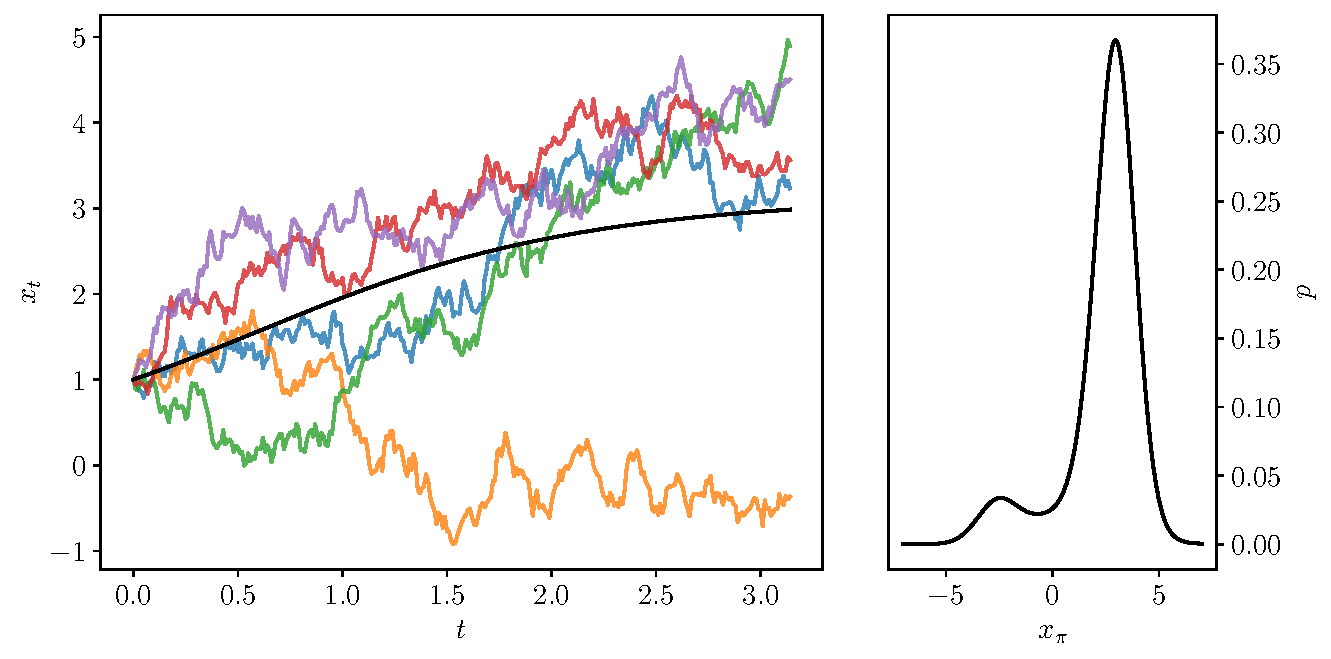
\includegraphics[width=\textwidth]{chp02_background/figures/ou_solution.pdf}
		\caption{(Left) Sample paths of the solution to the stochastic differential equation \(\dif x_t = \sin\!\left(x_t\right)\dif t + \dif W_t\), from the initial condition \(x_0 = 1\) and over the time interval \((0,\pi)\).
			The solution to the corresponding deterministic system \(\od{w_t}{t} = \sin\!\left(w_t\right)\) with the same initial condition is in black.
			(Right) The numerically estimated probability density function of the solution \(x_\pi\), using 10000 samples.}
		\label{fig:sde_sol_sample}
	\end{center}
\end{figure}

As an example, in \Cref{fig:sde_sol_sample} we show 10 realisations of the solution to the SDE \(\dif x_t = \sin\!\left(x_t\right)\dif t + \dif W_t\).
At any given time \(t\), the solution \(x_t\) follows a probability distribution over \(\R\), the (numerically estimated---see \Cref{sec:numeric_sdes}) probability density function of which is shown at \(t = \pi\) on the right-hand side of \Cref{fig:sde_sol_sample}.
Although the deterministic dynamics can give a loose indication of the behaviour of the stochastic samples, even additive noise can result in complicated behaviour in the stochastic system and departures from the deterministic solutions when the drift is nonlinear, evidenced by the trajectory (in orange) that clearly deviates from the deterministic one.


% Stochastic differential equations also arise as the limit of deterministic slow-fast systems, where the average behaviour of the `fast' dynamics can be shown to converge to the solution of a stochastic differential equation \citep[e.g.]{WongZakai_1965_ConvergenceOrdinaryIntegrals,MelbourneStuart_2011_NoteDiffusionLimits,GottwaldMelbourne_2013_HomogenizationDeterministicMaps}\lb{Maybe some better citations out there.}.
% A review of this theory is provided by \citet{GivonEtAl_2004_ExtractingMacroscopicDynamics}.
% This is particular relevant in climate and physics applications, where \citep{FranzkeEtAl_2015_StochasticClimateTheory}.
% This leads to stochastic parameterisation \citep{BernerEtAl_2017_StochasticParameterizationNew,Palmer_2019_StochasticWeatherClimate}, which we review in more detail in \Cref{sec:stoch_param}.

% The noise driving stochastic differential equations need not be a Wiener process, and can be instead replaced by any semi-martingale, which are a general class of stochastic processes.
% However, we primarily use the Wiener process throughout this thesis due to the aforementioned properties that make it appropriate for modelling scenarios and the ubiquitous use of it across literature and applications.
% We do briefly discuss the possibility of extending some of our work to L\'evy processes, a  more general class of stochastic processes, in \Cref{sec:disc_levy}.



\subsection{Numerical schemes for approximating SDEs}\label{sec:numeric_sdes}
In general, solving a stochastic differential equation analytically is not possible, and so as with ordinary differential equations we instead look to use numerical schemes to approximate solutions.
However, the solution to a stochastic differential equation is itself a random variable, so a single sample path is not sufficient.
Instead, a numerical SDE scheme involves random sampling (typically of the driving noise process) and produces approximate \emph{realisations} of the solution.
With a large number of these Monte Carlo realisations, one can estimate statistical properties and approximate the distribution of the solution.
The stochastic sampling approach is the gold-standard in many applications, most notably climate and weather modelling \citep{Collins_2007_EnsemblesProbabilitiesNew}.

The simplest scheme for numerically solving SDEs is the Euler-Maruyama (EM) method, which is analogous to the Euler method for ODEs \citep{KloedenPlaten_1992_NumericalSolutionStochastic}.
The update step of the EM scheme, with step size \(\delta t\), is
\begin{equation}
	\hat{x}_{t + \delta t} = \hat{x}_{t} + \delta t u\!\left(\hat{x}_t, t\right) + \sqrt{\delta t} \sigma\!\left(\hat{x}_t, t\right) Z_t,
	\label{eqn:em_step}
\end{equation}
where \(Z_t\) is sampled from the standard Gaussian \(\Gauss{0,I}\), and the scheme is initialised as \(\hat{x}_0 = x_0\).
When the initial condition is random, one samples \(\hat{x}_0\) from that distribution.
% The Euler-Maruyama scheme has strong order 0.5, meaning that
% \[
% 	\avg{\norm{x_t - \hat{x}_{t}\left(\Delta t\right)}} = \mathcal{O}\left(\Delta t^{0.5}\right),
% \]
% where \(\hat{x}_t\left(\Delta t\right)\) is the Euler-Maruyama estimate at time \(t\) using step size \(\Delta t\).
There are many other schemes for generating approximate samples of a stochastic differential equation, of varying precision and computational complexity, many of which are given in \citet{KloedenPlaten_1992_NumericalSolutionStochastic}.
Numerical schemes give us access to approximate solutions to otherwise intractable SDEs.
However, this comes at a computational cost: a large number of samples paths is often required to generate convergent statistics and make accurate inferences.
One of the primary aims of this thesis is to overcome this expense, by devising alternative ways of approximating and characterising SDE solutions that are computationally cheaper.






% \subsection{The Fokker-Planck equation}\label{sec:fp_eqn}
% The Fokker-Planck (FP) equation is a partial differential equation that describes the time evolution of the probability density function of the solution to a stochastic differential equation.
% The probability density function \(\rho: \R^n \times [0,T] \to [0,\infty)\) for the solution to \cref{eqn:gen_sde} at time \(t \in [0,T]\) is the solution to the corresponding Fokker-Planck equation \citep{Risken_2012_FokkerPlanckEquationMethods}
% \begin{equation}
% 	\dpd{\rho}{t} = \frac12\nabla\cdot\nabla\cdot\left(\rho\sigma\sigma^{\T}\right) - \nabla\cdot\left(\rho u\right)
% 	\label{eqn:fp_eqn}
% \end{equation}
% subject to some initial density \(\rho\left(x,0\right)\) given by the initial condition to \cref{eqn:gen_sde}.
% For a fixed and deterministic initial condition \(y_0 = x\), the corresponding initial condition to \cref{eqn:fp_eqn} is the Dirac-delta distribution centred at \(x\).
% To ensure that the solution is a valid probability density function on \(\R^n\), for any \(t \in [0,T]\), \(\rho\) must satisfy
% \begin{subequations}\label{eqn:fp_valid_pdf}
% 	\begin{align}
% 		\int_{\R^n}{\rho\left(x, t\right)\dif x} = 1, \label{eqn:fp_valid_pdf_norm} \\
% 		\lim_{x \to \infty}\rho\left(x,t\right) = 0. \label{eqn:fp_valid_pdf_limit}
% 	\end{align}
% \end{subequations}
% Solving the Fokker-Planck equation provides an alternative method for finding the solution to a stochastic differential equation; rather than dealing with stochastic quantities, we instead seek solutions to the
% However, the Fokker-Planck equation cannot be solved analytically except for simple cases and there are several practical difficulties in attempting to solve it numerically.
% These difficulties include:
% \begin{itemize}
% 	\item \textbf{Dimensionality:} In high-dimensional systems, solving the Fokker-Planck equation numerically is computationally prohibitative, requiring a small spatial discretisation to be accurate.
% 	\item \textbf{Boundary conditions:} The Fokker-Planck equation is often defined on an unbounded domain with the zero-limit constraint \cref{eqn:fp_valid_pdf_limit}, which presents computational difficulties.
% 	\item \textbf{Normality constraints:} The Fokker-Planck equation must be solved with the additional normality condition \cref{eqn:fp_valid_pdf_norm}, which enforces an additional constraint on any numerical solution.
% \end{itemize}
% It is generally accepted that these difficulties mean that the computational cost of solving the Fokker-Planck equation is too high in \(3\)- or higher dimensions \citep{ZhaiEtAl_2022_DeepLearningMethod,Li_2019_DatadrivenMethodSteady,AllawalaMarston_2016_StatisticsStochasticallyForced}.

% \td{Perhaps comment on how the FP equation arises in other settings, and is a generalisation of the advection-diffusion equation and similar. Hence learning stuff about the solution to the SDE also tells us about the FP equation.}

% \subsubsection{Relationship to the classical advection-diffusion equation}
% The advection-diffusion equation describes the time-evolution of a passive and inert scalar quantity, such as temperature, salinity

% \citep{Visser_2008_LagrangianModellingPlankton}

% Let \(c \colon \Omega_0 \times [0,T] \to [0, \infty)\) denote the concentration of a passive and inert scalar quantity, then the classical advection-diffusion equation is
% \begin{equation}\label{eqn:advec_diff}
% 	\dpd{c}{t} = - \nabla\cdot \left(v\!\left(x,t\right)c\!\left(x,t\right)\right) + \nabla\cdot\left(K\!\left(x,t\right)\nabla c\!\left(x,t\right)\right), \quad c\!\left(x,0\right) = c_0\!\left(x\right),
% \end{equation}
% where \(v\) denotes the flow velocity dictating the advection (displacement) of the tracer, and \(K\) is a matrix describing the diffusion (dispersion) of \(c\).




% If we set \(u\!\left(x,t\right) = v\!\left(x,t\right) + \nabla \cdot K\!\left(x,t\right)\) and \(\sigma\!\left(x,t\right)\sigma\!\left(x,t\right) = K\!\left(x,t\right)\), then the Fokker-Planck equation \cref{eqn:fp_eqn} is equivalent to the advection-diffusion equation \cref{eqn:advec_diff}.
% Thus, the evolution of the tracer concentration under \cref{eqn:advec_diff} can be equivalently considered as the probability density function of solutions to the stochastic differential equation
% \begin{equation}\label{eqn:ad_sde}
% 	\dif x_t = \left[u\!\left(x_t, t\right) + \nabla \cdot K\!\left(x_t, t\right)\right]\dif t + \kappa\!\left(x_t, t\right)\dif W_t, \quad x_t \sim \hat{c}_0,
% \end{equation}
% where \(\kappa\) is any matrix-valued function satisfying \(K \equiv \kappa\kappa^{\T}\), and
% \[
% 	\hat{c}_0\!\left(x\right) = \frac{c_0\!\left(x\right)}{\int_{\Omega_0}c_0\!\left(z\right)\dif z},
% \]
% is the initial density of \cref{eqn:advec_diff} normalised to describe a probability density function.
% Assuming that the total concentration tracer is conserved, that is
% \[
% 	\int_{\Omega_t}{c\!\left(z,t\right)\dif z} = \int_{\Omega_0}{c_0\!\left(z\right)\dif t}
% \]
% for all \(t \in [0,T]\), then we can recover \(c\) from the probability density function \(\rho\) corresponding to \cref{eqn:ad_sde} as
% \[
% 	c\!\left(x,t\right) = \rho\!\left(x,t\right)\int_{\Omega_0}{c_0\!\left(z\right)\dif t}.
% \]
% An implication of this connection is that the theory and computations for stochastic differential equations developed throughout this thesis can be applied to \emph{any} scalar field that is modelled with an advection-diffusion type equation.


% \subsubsection{Green's function method}
% The Fokker-Planck equation is linear, so we can apply a technique known as Green's function method (for an example of this approach on a linear SDE, see Section 3.2 of \citet{Risken_2012_FokkerPlanckEquationMethods}) in order to understand the behaviour of solutions with non-fixed initial conditions.
% Let \(\mathcal{P}_t\set{\rho_0}\) denote the solution operator of \cref{eqn:fp_eqn} with initial density \(\rho_0\colon \R^n \to \R^n\).
% Then, since \cref{eqn:fp_eqn} is a linear equation, \(\mathcal{P}_t\) is a linear operator.
% Now, let \(x_0 \in \R^n\) be an arbitrary fixed point, and consider the fundamental solution, or Green's function,
% \[
% 	G_t\left(x; x_0\right) \coloneqq \mathcal{P}_t\set{\delta_{x_0}}\!\left(x\right).
% \]
% That is, \(G_t\left(x; x_0\right)\) is the solution to the Fokker-Planck equation with the Dirac-delta initial condition \(\delta_{x_0}(x) = \delta\left(x - x_0\right)\), which is equivalent to the SDE \cref{eqn:gen_sde} with the deterministic and fixed initial condition \(y_0 = x_0\).
% The Green's function \(G_t\) is equivalently the transition probability function of the SDE solution \(x_t\) as a stochastic process.
% Now, using the sampling property of the Dirac-delta function, for a general initial density \(\rho_0\colon \R^n \to \R^n\),
% \[
% 	\rho_0(x_0) = \int_{\R^n}{\rho_0\left(x\right)\delta_{x_0}\left(x\right)\dif x}.
% \]
% Since \(\mathcal{P}_t\) is linear,
% \begin{equation}
% 	\mathcal{P}_t\set{\rho_0}\!\left(x_0\right) = \int_{\R^n}{\rho_0\!\left(x\right)\mathcal{P}_t\set{\delta_{x_0}}\!\left(x\right)\dif x} = \int_{\R^n}{\rho_0\!\left(x\right) G_t\!\left(x; x_0\right)\dif x}.
% 	\label{eqn:fp_greens_trick}
% \end{equation}
% An implication of \cref{eqn:fp_greens_trick} is that for a given stochastic differential equation, we only need to understand the behaviour of solutions subject to a fixed (albeit arbitrary) initial condition.


\section{Lagrangian coherent structures}\label{sec:bkg_lcs}

\begin{figure}
	\begin{center}
		\begin{subfigure}[t]{0.49\textwidth}
			\includegraphics[width=\textwidth]{chp02_background/figures/dwh_cropped}
			\caption{An oil slick from the \emph{Deepwater Horizon} oil spill in 2010 (NASA Image of the Day, May 19, 2010).
				The southwards extension of the slick appeared unexpectedly.}
			\label{fig:lcs_deepwater}
		\end{subfigure}
		\begin{subfigure}[t]{0.49\textwidth}
			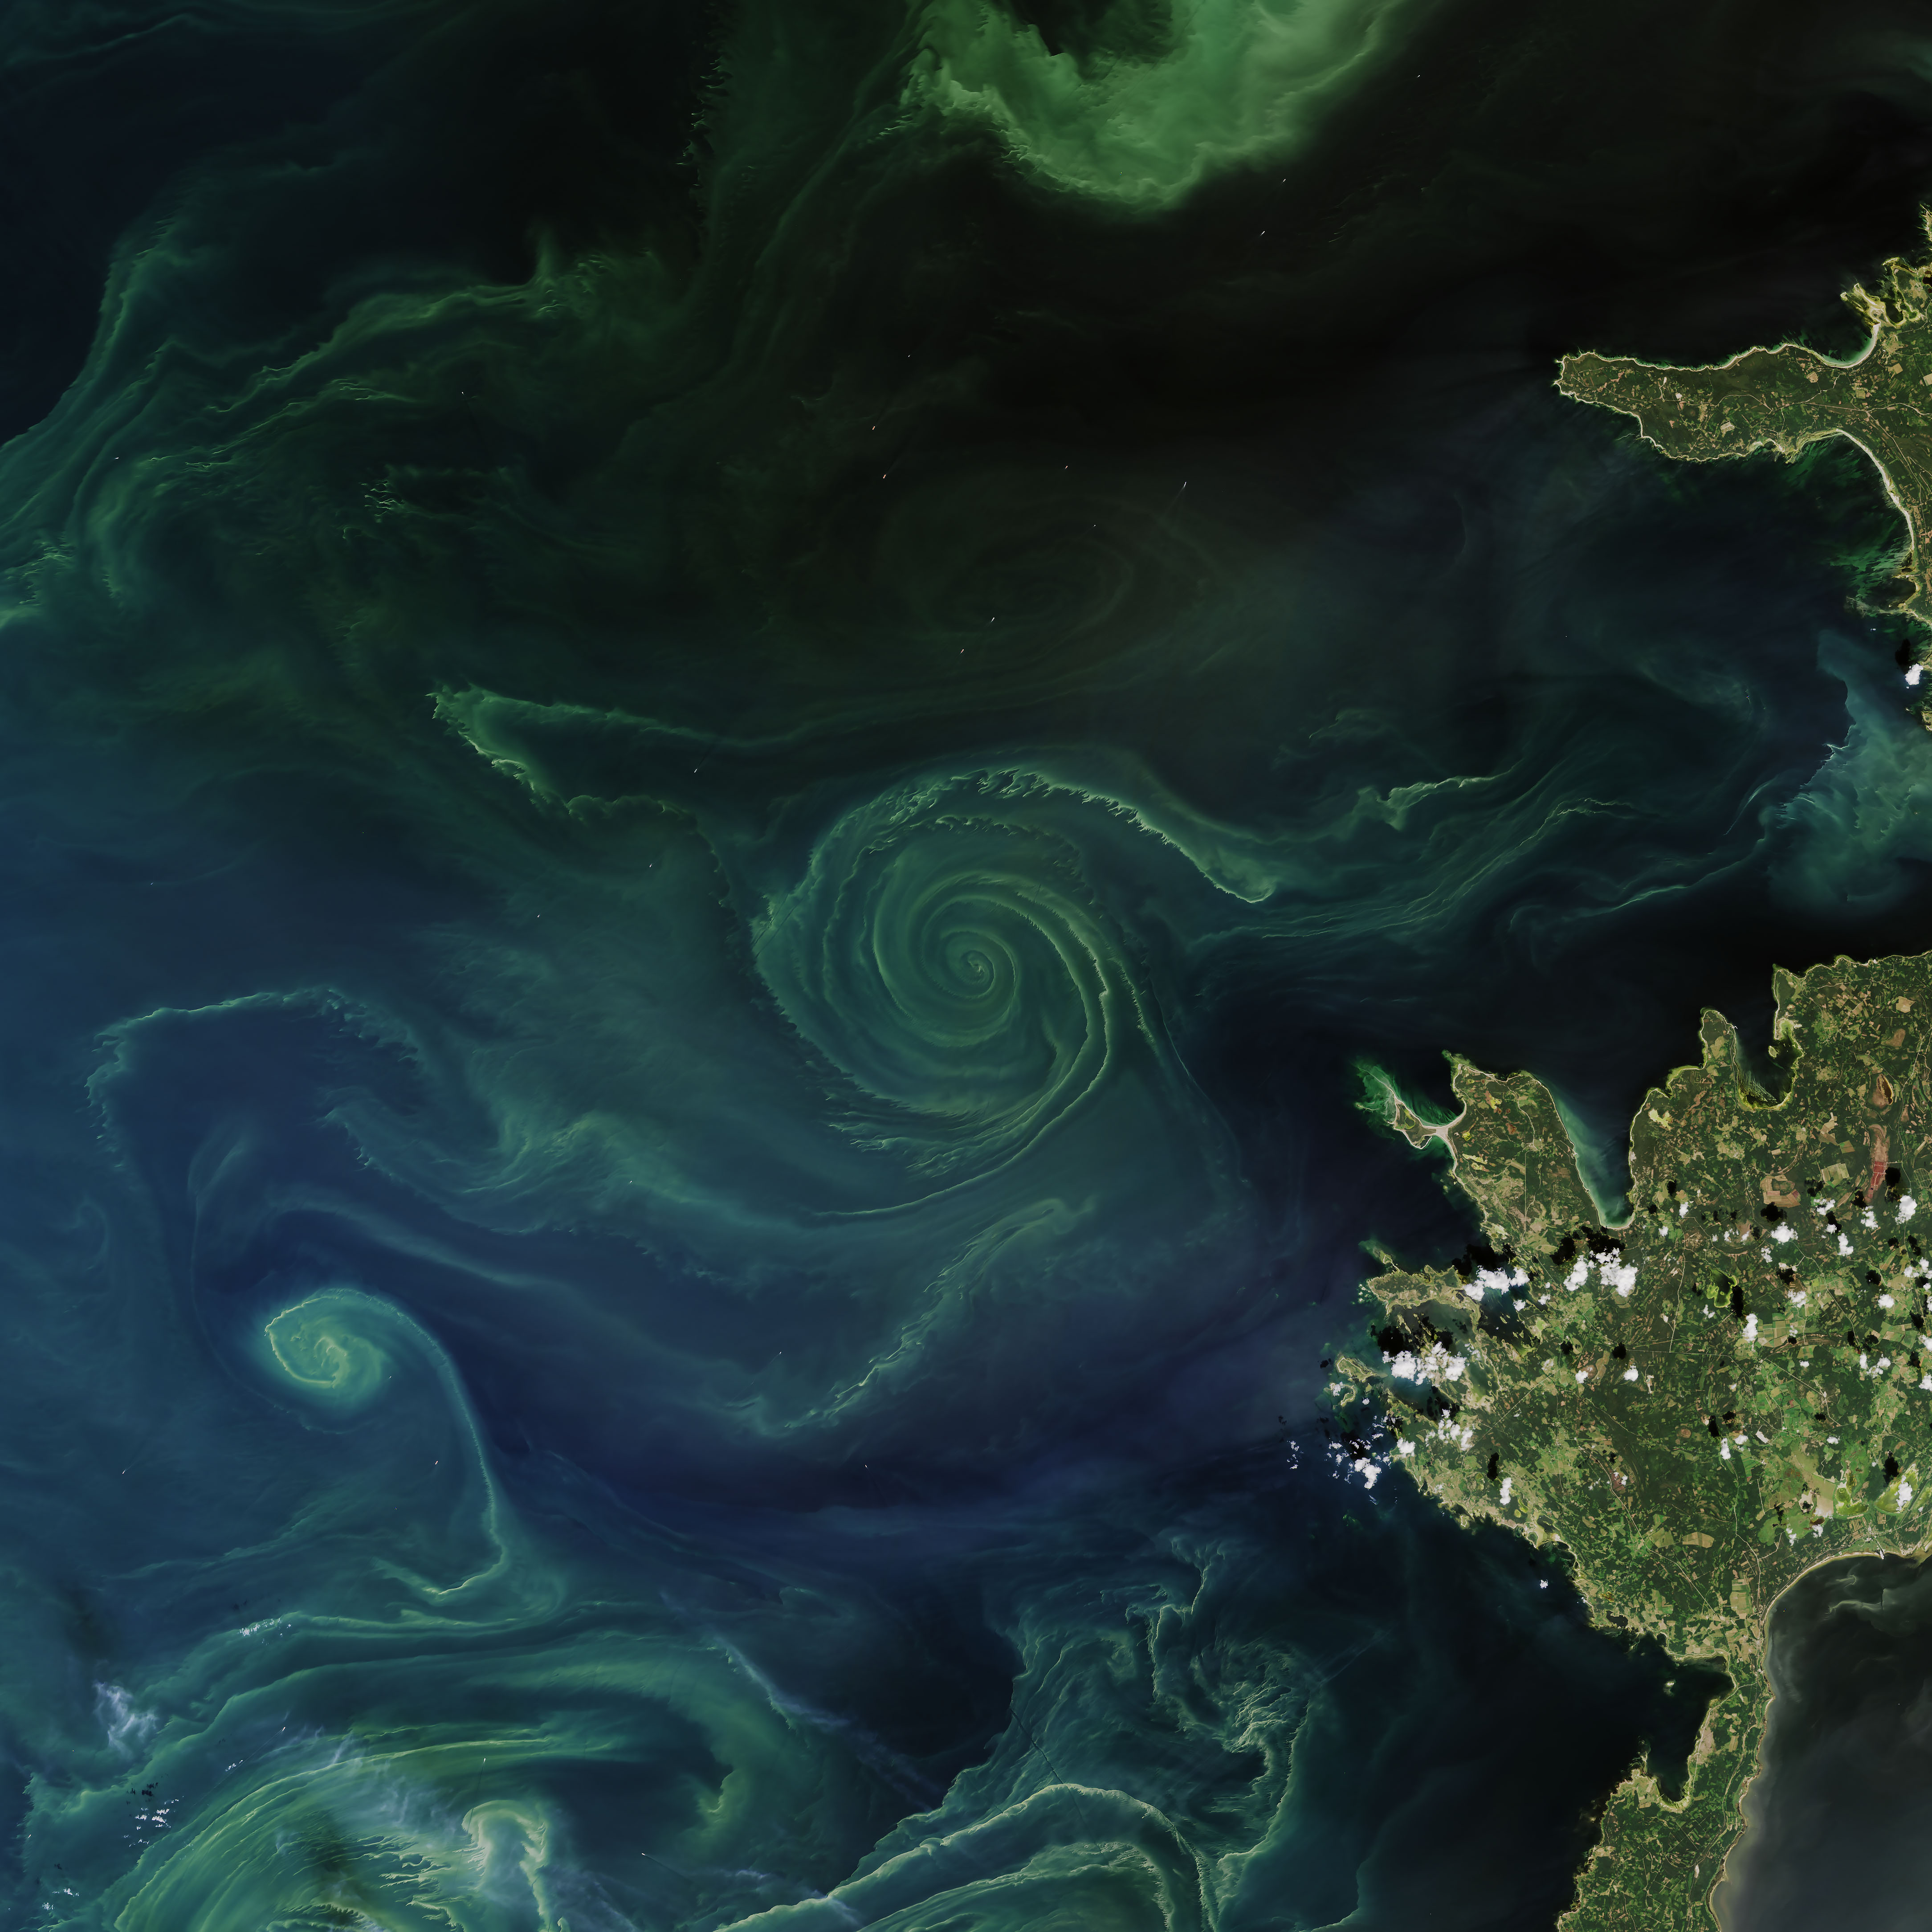
\includegraphics[width=\textwidth]{chp02_background/figures/photoplankton}
			\caption{Phytoplankton blooms in the Baltic Sea (NASA Earth Observatory, July 18, 2018).
				The structure of these blooms reflect the underlying flow of the Sea.}
			\label{fig:lcs_phyto}
		\end{subfigure}
		\begin{subfigure}[t]{\textwidth}
			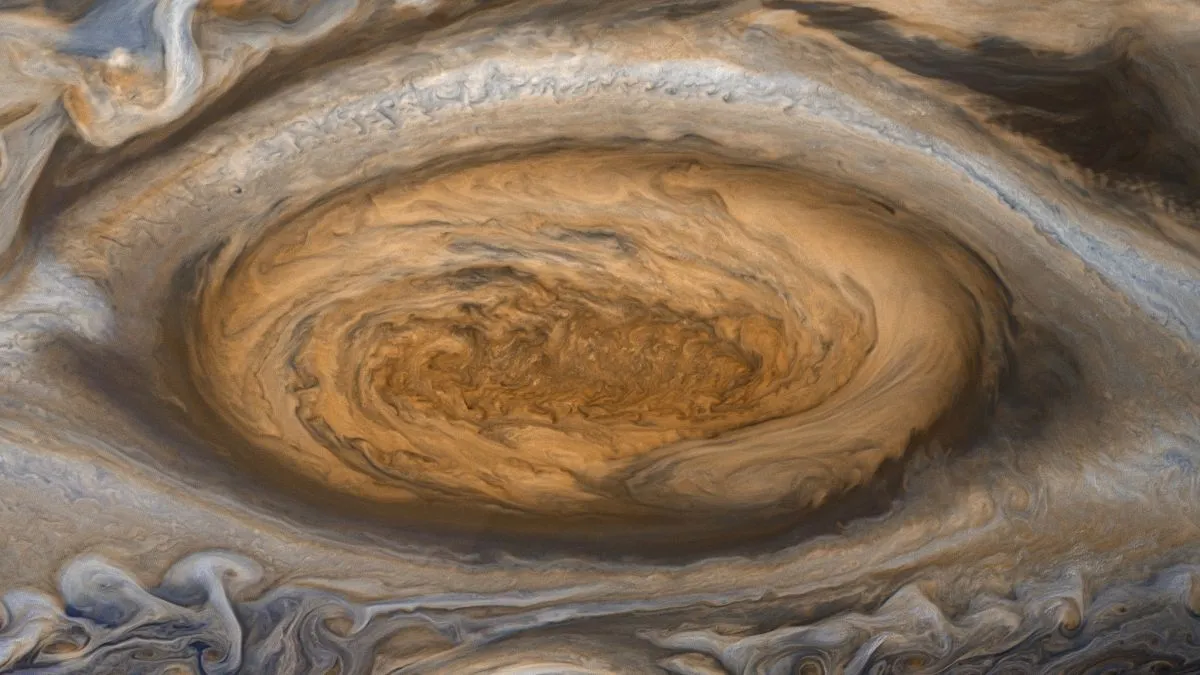
\includegraphics[width=\textwidth]{chp02_background/figures/red_spot.png}
			\caption{Jupiter's Great Red Spot, as photographed by the Voyager 1 probe (NASA/JPL-Caltech and processed by Bj\"{o}rn J\'{o}nsson, March 5, 1979).
			The storm is an example of a vortex or eddy within the atmospheric flow of the planet.}
		\end{subfigure}
		% \begin{subfigure}[t]{0.49\textwidth}
		% 	% 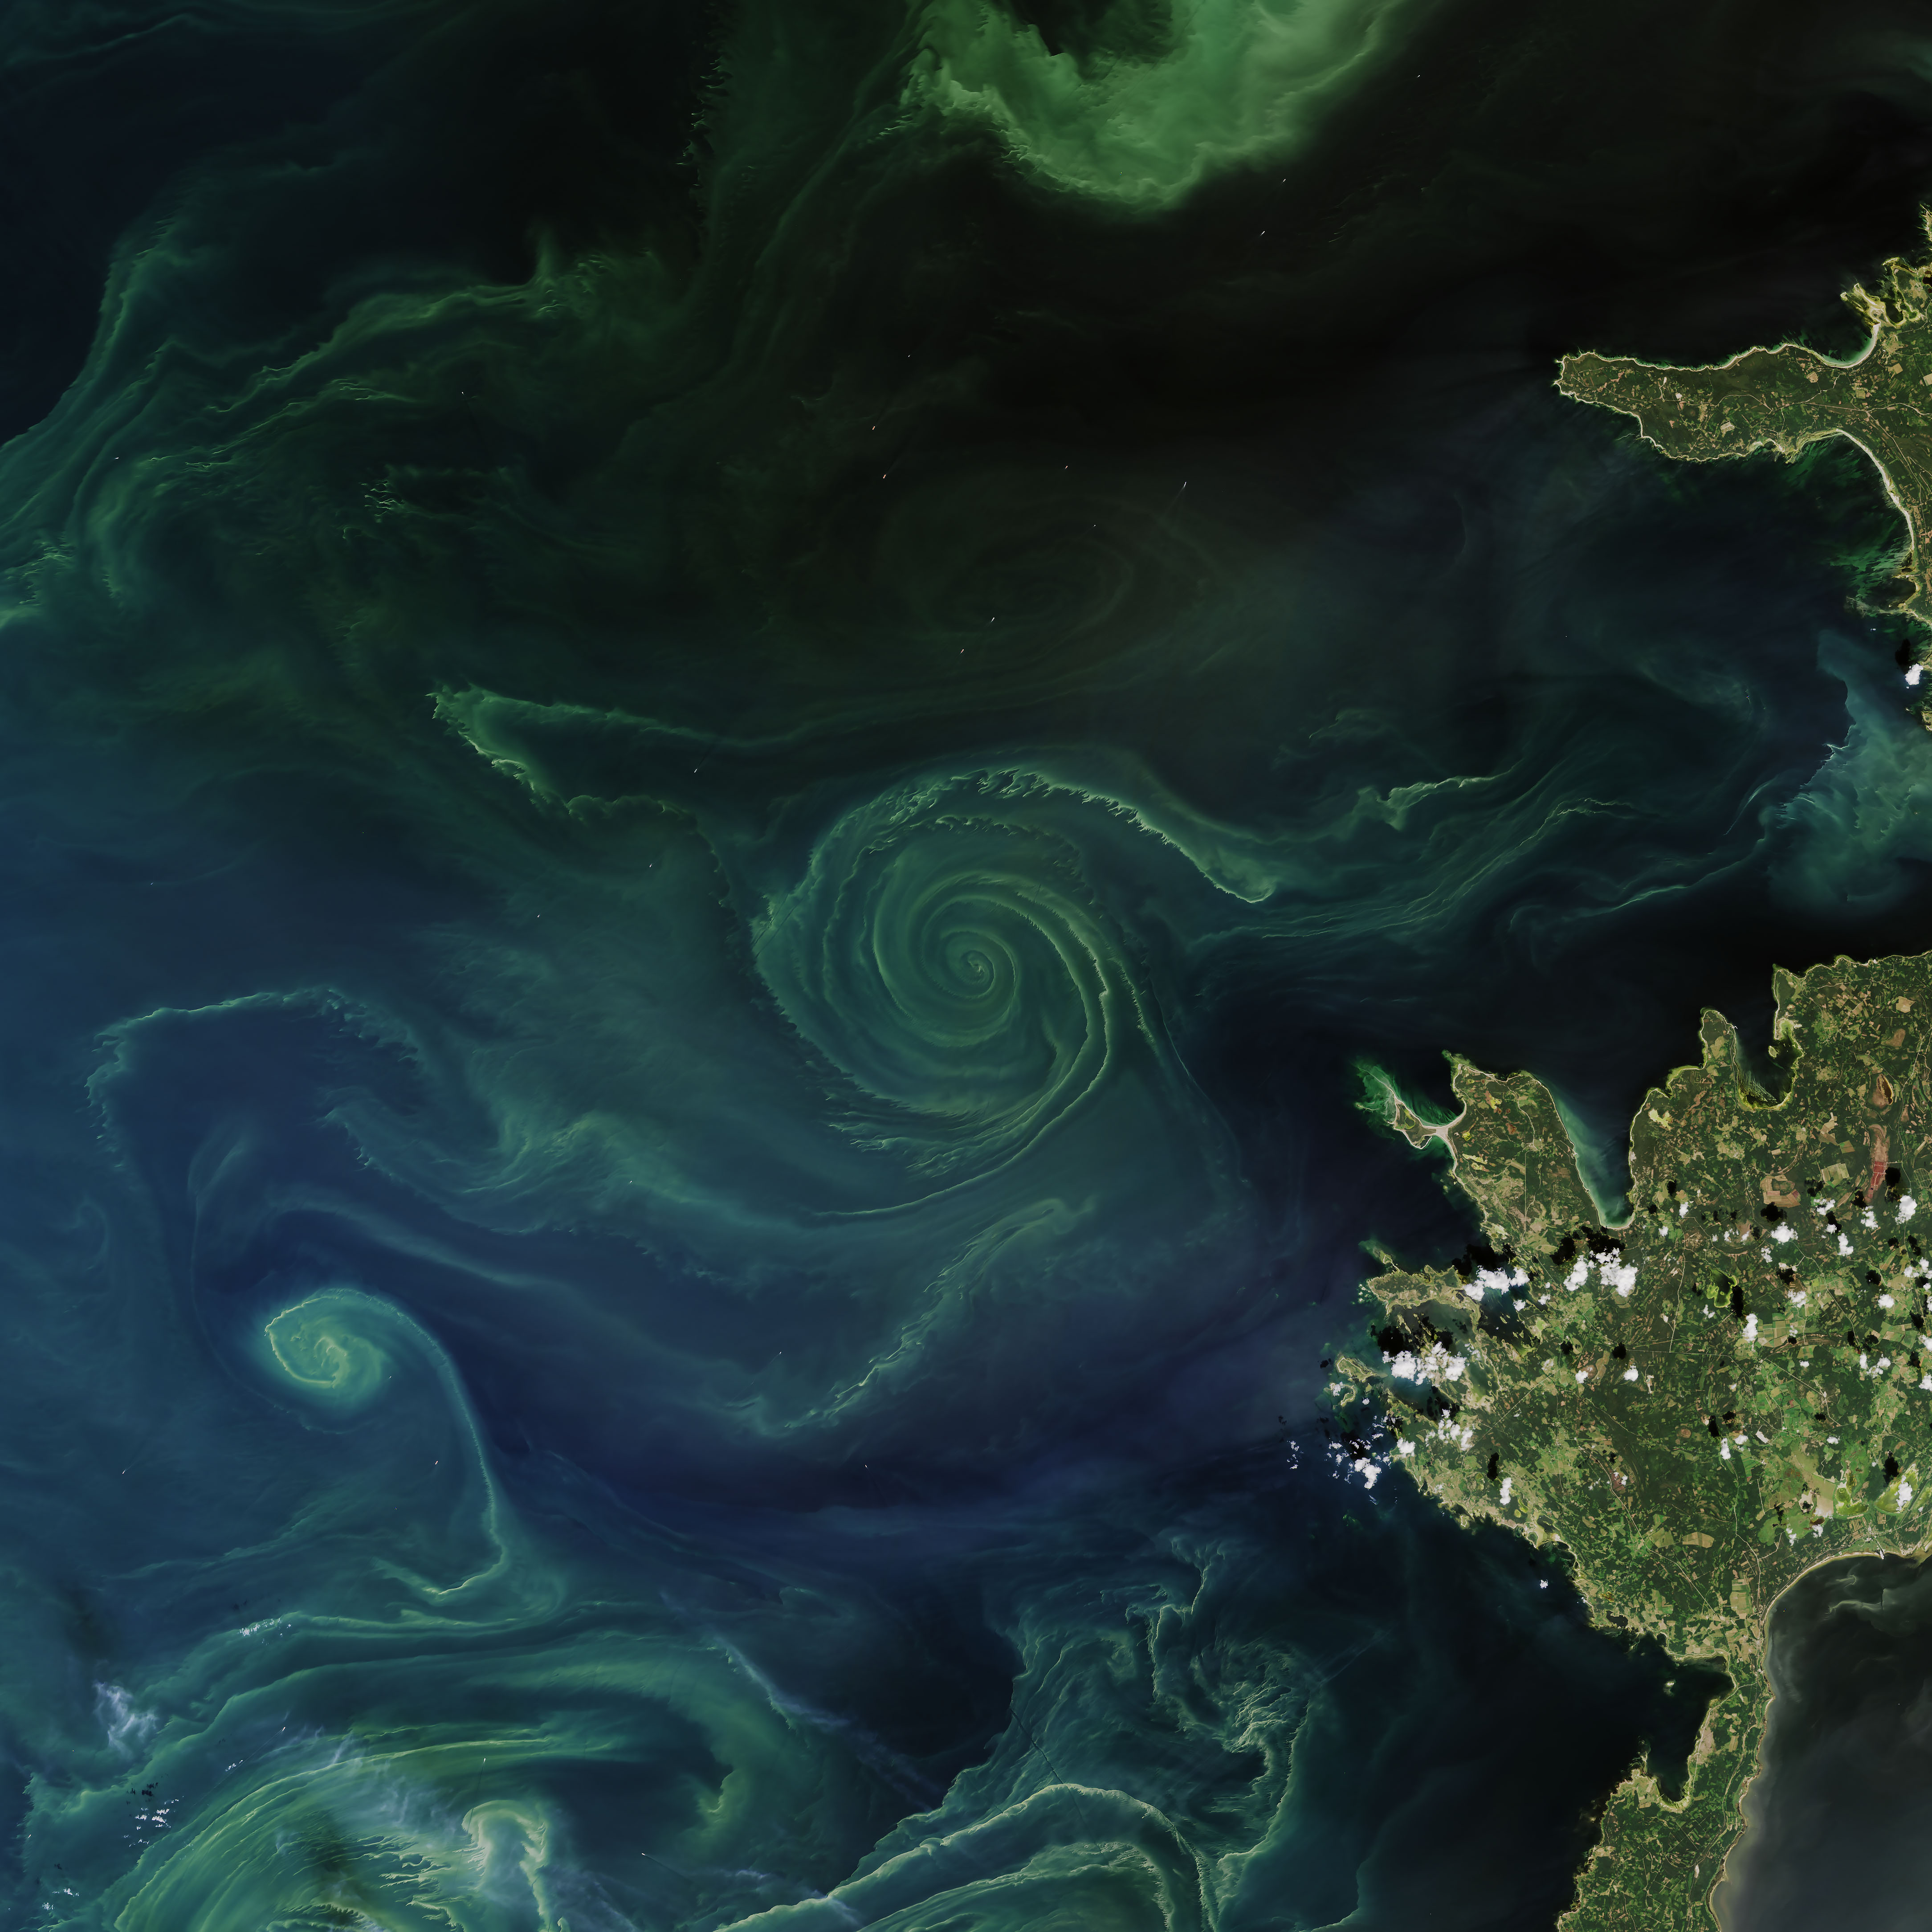
\includegraphics[width=\textwidth]{chp02_background/figures/photoplankton}
		% 	\td{Get one more example!}
		% 	\caption{}
		% \end{subfigure}
		\caption{Examples of coherent patterns emerging in fluid flows observed in nature.}
		\label{fig:lcs_examples}
	\end{center}
\end{figure}

In this section, we take a brief sojourn into the field of Lagrangian coherent structures (LCSs), which provide qualitative insight into the behaviour of a dynamical system, particularly in the context of fluid flows.
Although LCSs are not the primary focus of this work, the field provides potential applications for our uncertainty quantification, that builds upon preliminary work by \citet{Balasuriya_2020_StochasticSensitivityComputable,Balasuriya_2020_UncertaintyFinitetimeLyapunov} and \citet{BadzaEtAl_2023_HowSensitiveAre}.
There is no universally accepted definition of a coherent structure, but typically these are structures within a flow that remain together over the time-evolution of the system and separate the spatial domain into regions with qualitatively different behaviour \citep{BalasuriyaEtAl_2018_GeneralizedLagrangianCoherent}.
\Cref{fig:lcs_examples} show examples of coherent structures in observed fluid flows, which can be considered LCSs.
These are structures such as vortices, eddies, and jets that influence the transport of material within the fluid.
For instance, in \Cref{fig:lcs_deepwater,fig:lcs_phyto} the observed patterns of the oil slick and phytoplankton blooms respectively reflect the behaviour of the underlying ocean flow and are influenced by jet- and eddy-like structures.

In a steady system (that is, the vector field \(u\) in \cref{eqn:det_ode} is independent of time), we can gain this insight by using classical methods in dynamical systems, such as phase portrait analysis and identifying unstable and stable manifolds.
For example, unstable and stable manifolds cannot be intersected by solution trajectories, and so can act as barriers for the transport of material within a flow.
However, when the system is non-autonomous (that is, the vector field explicitly depends on time \(t\)), these structures can themselves vary with time and the problem of identifying them is far more non-trivial.
Another complication is that in practice the data driving a system is only available over a finite timeframe, whereas classical dynamical systems techniques often tell us about the long-term (in the infinite time limit) behaviour of solutions.
Lagrangian coherent structure theory provides a mathematical framework for defining and identifying such structures within a given flow \citep{BalasuriyaEtAl_2018_GeneralizedLagrangianCoherent}.
There are many procedures and heuristics for extracting these regions from a given flow, which draw upon different mathematical techniques, including classical dynamical system theory, variational calculus, transfer operators, and statistical clustering.
Detailed reviews of approaches to Lagrangian coherent structure extraction are provided by \citet{PeacockDabiri_2010_IntroductionFocusIssue}, \citet{HadjighasemEtAl_2017_CriticalComparisonLagrangian}, and \citet{BalasuriyaEtAl_2018_GeneralizedLagrangianCoherent}.

Coherent structures can provide valuable qualitative insight into the behaviour of a flow, by providing an outline of the transport properties and underlying dynamics.
An example is in the study of the spread of the oil slick resulting from the 2010 Deepwater Horizon disaster in the Gulf of Mexico (see \Cref{fig:lcs_deepwater}).
Investigations showed that the behaviour of the slick, including a sudden and unexpected extension of the slick, could be understood and therefore predicted in future cases by using Lagrangian coherent structures and the insight they provide \citep{OlascoagaEtAl_2013_DrifterMotionGulf,OlascoagaHaller_2012_ForecastingSuddenChanges,MezicEtAl_2010_NewMixingDiagnostic}.
This approach explained dynamics that were otherwise poorly understood due to the time-varying and complex nature of the flow.

One of the most well-studied and frequently used procedures for extracting Lagrangian coherent structures is via the finite-time Lyapunov exponent (FTLE), which is a measure quantifying the stretching of infinitesimal regions of the flow over a time period.
The FTLE can be computed as a scalar field over a set of initial conditions, from which the maximising ridges can correspond to flow barriers \citep{ShaddenEtAl_2005_DefinitionPropertiesLagrangian}.
Importantly, the finite-time Lyapunov exponent can be computed only using the gradients of the flow map, which ensures a highly practical and flexible procedure that can be used across many different contexts.
The FTLE is an example of a common class of LCS methods that first compute a field over a set of initial conditions and then extracts coherent structures based on that field.

% One of the best known procedures for extracting LCSs is via the finite-time Lyapunov exponent (FTLE) \citep{ShaddenEtAl_2005_DefinitionPropertiesLagrangian}, which is a measure quantifying the stretching of infinitesimal regions of a flow over a finite time period.
% Take an initial condition \(x\) and let \(F_0^t\) represent the flow map of our system over the time interval \([0,t]\).
% We wish to quantify the impact of a small change in the initial condition on the flow at time \(t\), so take \(\delta\) as a small and arbitrary perturbation to \(x\).
% Then, we measure the \emph{stretching} in the direction of \(\delta\) with
% \[
% 	s\!\left(x, \delta\right) = \frac{\norm{F_0^t\!\left(x + \delta\right) - F_0^t\!\left(x\right)}}{\norm{\delta}}
% \]
% For sufficiently small \(\delta\), we can replace the mapped perturbation with a linearisation of the flow map about \(x\), that is
% \[
% 	s\!\left(x, \delta\right) \approx \frac{\norm{\nabla F_0^t\!\left(x\right) \delta}}{\norm{\delta}}.
% \]
% % \Cref{fig:ftle_illustr} provides a pictorial representation of this calculation; a small !!!!!
% Taking the supremum over all possible perturbations \(\delta\), we have
% \[
% 	\sup_{\delta \in \R^n, \, \delta \neq 0}s\!\left(x, \delta\right) \approx \norm{\nabla F_0^t\!\left(x\right)},
% \]
% which quantifies the stretching about the trajectory \(F_0^t\!\left(x\right)\).
% The finite-time Lyapunov exponent is then computed as
% \begin{equation}
% 	\mathrm{FTLE}_0^t\!\left(x\right) = \frac{1}{\abs{t}}\ln\!\left(\norm{\nabla F_0^t\!\left(x\right)}\right).
% 	\label{eqn:ftle_defn}
% \end{equation}
% Note that the operator norm \(\norm{\nabla F_0^t\!\left(x\right)}\) in \cref{eqn:ftle_defn} can be readily computed as the square root of the largest eigenvalue of the Cauchy-Green tensor \(\left[\nabla F_0^t\!\left(x\right)\right]^{\T}\nabla F_0^t\!\left(x\right)\).
% Over the set of initial conditions, the FTLE is a scalar field that measures for each initial condition the stretching and contraction along the resulting trajectory.
% The FTLE is a measure of exponential stretching (hence the scalings in \cref{eqn:ftle_defn}), and provides insight into the nonlinearity of a system, including as an indicator of one defining feature of chaos.
% It was shown by \citet{ShaddenEtAl_2005_DefinitionPropertiesLagrangian} that the maximising ridges of the FTLE field can correspond to flow barriers, and so by finding these ridges, one can extract coherent structures for the flow.


% In \Cref{fig:gs_lcs}, we compute the FTLE field of our Gulf Stream velocity model over a timespan of 7 days.



% \begin{figure}
% 	\begin{center}
% 		\begin{subfigure}{0.49\textwidth}
% 			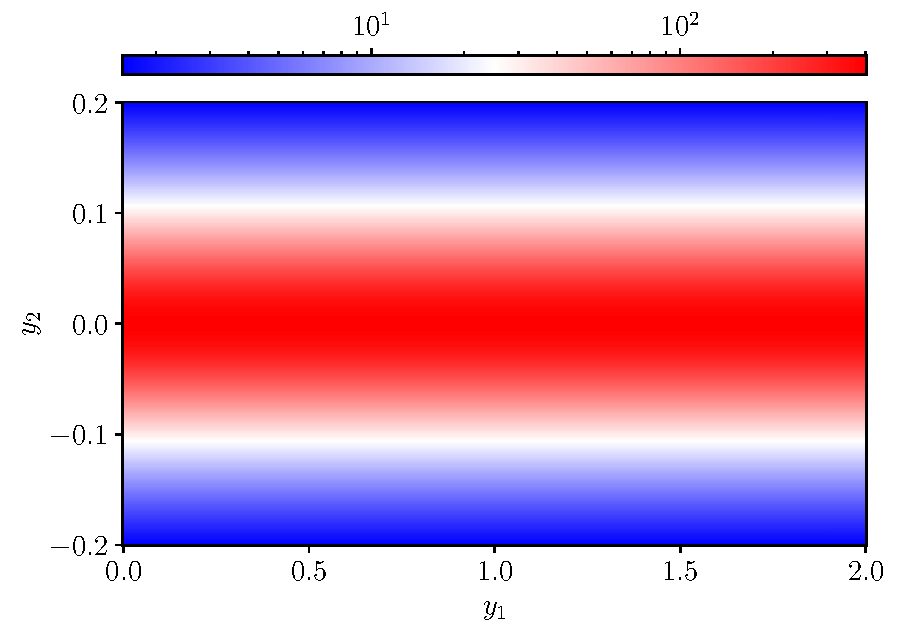
\includegraphics[width=\textwidth]{chp02_background/figures/gulf_stream_motivation/ftle.pdf}
% 			\caption{The finite-time Lyapunov exponent field.}
% 		\end{subfigure}
% 		\begin{subfigure}{0.49\textwidth}
% 			\caption{Maximising ridges of the FTLE field.}
% 		\end{subfigure}
% 		\caption{The finite-time Lyapunov exponent field computed, and corresponding maximising ridges.
% 			This is an example of using a scalar field to extract Lagrangian coherent structures from a fluid flow.
% 			The resulting maximises ridges indicate a skeleton of the Gulf Stream.}
% 		\label{fig:gs_lcs}
% 	\end{center}
% \end{figure}


Most well-established LCS frameworks and extraction procedures are purely deterministic, in that they are defined and computed solely in terms of the behaviour of the underlying ordinary differential equation.
However, uncertainty in such systems is inevitable in practice and these methods fail to explicitly account for this.
Accordingly, there is an emerging interest \citep{Balasuriya_2020_StochasticApproachesLagrangian} in extending LCS theory to stochastic settings.
There are two primary ways in which stochastic has been recently investigated in the LCS community:
\begin{romanate}
	\item in creating novel procedures that explicitly account for such ongoing uncertainty, such as by using properties of corresponding stochastic systems.
	For example, see (in \Cref{sec:s2_summ}) stochastic sensitivity introduced by \citet{Balasuriya_2020_StochasticSensitivityComputable}, model sensitivity introduced by \citet{KaszasHaller_2020_UniversalUpperEstimate}, and the finite-time divergence rate by \citet{BranickiUda_2023_PathBasedDivergenceRates}.
	These are scalar fields defined on initial conditions that measure the certainty in the corresponding deterministic trajectories and can be used to extract coherent regions in similar ways to deterministic methods.
	As another example, \citet{DennerEtAl_2016_ComputingCoherentSets} directly compute coherent sets by working with a discretised Fokker-Planck equation, which is a partial differential equation that governs the probability density function of an SDE solution (a brief overview is provided in \Cref{sec:disc_fp}).
	This Fokker-Planck approach extends the transfer operator method of \citet{Froyland_2013_AnalyticFrameworkIdentifying}, which is a popular method for LCS detection and extraction by encoding how densities are pushed forward by the flow.
	Until recently the transfer-operator, at least in the context of Lagrangian analysis, has been viewed as purely deterministic but provides a framework for naturally including velocity field uncertainties that is only recently being explored \citet{Balasuriya_2020_StochasticApproachesLagrangian}.

	\item in understanding the direct impact of velocity uncertainty on well-established deterministic LCS measures.
	\citet{BadzaEtAl_2023_HowSensitiveAre} provide a systematic analysis, using Monte Carlo simulation and summary statistics to evaluate the robustness of several common LCS extraction schemes to velocity uncertainty.
	% It is shown that LCS methods that directly account for this uncertainty, such as stochastic sensitivity \citep{Balasuriya_2020_StochasticSensitivityComputable}, are the most robust.
	The finite-time Lyapunov exponent has received particular attention, with recent studies aiming to quantify the impact of velocity field uncertainty on the FTLE computation: \citet{GuoEtAl_2016_FiniteTimeLyapunovExponents} use stochastic simulation and statistical analysis, \citet{Balasuriya_2020_UncertaintyFinitetimeLyapunov} provides theoretical error bounds on the FTLE computation, and \citet{YouLeung_2021_ComputingFiniteTime} propose an approach for computing the (statistically) expected FTLE field.

\end{romanate}
In this thesis, we are primarily interested in point (i), by exploring how our characterisations of uncertainty can be applied to extract coherent structures.
This is directly extending the stochastic sensitivity of \citet{Balasuriya_2020_StochasticSensitivityComputable}, which is summarised in \Cref{sec:s2_summ}.
We will also discuss (in \Cref{ch:outlook}) how we anticipate our work could be applied to point (ii), as a quantification of uncertainty in computations involving the flow map in other LCS schemes.




\section{Stochastic sensitivity}\label{sec:s2_summ}
To conclude our background and motivation, this section provides a brief summary of stochastic sensitivity, a measure of uncertainty in differential equation introduced by \citet{Balasuriya_2020_StochasticSensitivityComputable}.
These tools are \emph{computable} given only velocity data, which enables an efficient quantification of uncertainty in a stochastic system without needing bulk simulation.
Stochastic sensitivity (also termed \(S^2\) in both notation and prose) was originally provided for 2-dimensional systems only, and the primary motivation was to understand the impact of velocity field uncertainty on fluid flows.
Given possibly time-dependent velocity data \(u\colon \R^2 \times [0,T] \to \R^2\), \citet{Balasuriya_2020_StochasticSensitivityComputable} considers the evolution of solutions to the ordinary differential equation
\begin{equation}\label{eqn:s2_ode}
	\dod{x_t}{t} = u\!\left(x_t, t\right),
\end{equation}
subject to some fixed initial condition \(x_0\).
The velocity field \(u\) is \emph{Eulerian}, in that it describes the fluid velocity at a given point in space and time.
The trajectories that solve \cref{eqn:s2_ode} are \emph{Lagrangian}, and correspond to the movement of idealised infinitesimal particles within the flow.
These Lagrangian trajectories are summarised by the flow map \(F_s^t\) of \cref{eqn:s2_ode}.
As we have continued to emphasise, the velocity field \(u\) is in practice subject to unavoidable uncertainties.
\citet{Balasuriya_2020_StochasticSensitivityComputable} aims to quantify the impact of this Eulerian uncertainty, directly attributed to \(u\), on the Lagrangian trajectories arising from integration of the velocity field.
% In most practical situations, the Eulerian velocity data driving ocean and atmospheric models relies upon measurements of estimates obtained on a low resolution spatial discretisation.
% \citet{Balasuriya_2020_StochasticSensitivityComputable} introduces stochastic sensitivity as a new tool for directly quantifying the impact of Eulerian uncertainty on Lagrangian trajectories.

To directly account for these unresolved sources of uncertainty, the ``true'' Lagrangian trajectories evolve as solution to the stochastic differential equation
\begin{equation}
	\sde{y_t}{u\!\left(y_t, t\right)}{\epsilon\sigma\!\left(y_t, t\right)}, \quad y_0 = x_0
	\label{eqn:s2_sde},
\end{equation}
where \(0 < \epsilon \ll 1\) is a parameter quantifying the scale of the noise, \(\sigma\colon	\R^2\times[0,T] \to \R^{2\times 2}\) is the \(2\times 2\) diffusion matrix, and \(W_t\) is the canonical 2-dimensional Wiener process.
In the original formulation \citep{Balasuriya_2020_StochasticSensitivityComputable}, \(\epsilon\) is a dimensionless parameter and \(\sigma\) is dimensional, but an alternative scaling technique relates \(\epsilon\) to spatial and velocity uncertainty scales in the data (see the follow-up work by \citet{Balasuriya_2020_UncertaintyFinitetimeLyapunov}, \citet{FangEtAl_2020_DisentanglingResolutionPrecision}, and \citet{BadzaEtAl_2023_HowSensitiveAre} for example).
Since \(\sigma\) can vary by both space and time, the noise is permitted to be multiplicative.
The diffusion matrix \(\sigma\) is specified \emph{a priori}, based on any knowledge of how uncertainty varies with space and time, e.g.\ from experimental considerations, observation error estimates, physics-informed models, etc.
If no such prior information is known, then \(\sigma \equiv I\), the \(2 \times 2\) identity matrix is the default choice.

Next, to quantify uncertainty at a time \(t\), \citet{Balasuriya_2020_StochasticSensitivityComputable} defined the random variable \(z_\epsilon\left(x_0\right)\) as
\[
	z_\epsilon\!\left(x_0\right) \coloneqq \frac{y_t - F_0^t\!\left(x_0\right)}{\epsilon},
\]
which captures the random deviation between the ``true'' stochastic trajectories and the deterministic flow map.
The aim was to compute statistics of \(z_\epsilon\).
To derive such quantities that can be computed in practice, \citet{Balasuriya_2020_StochasticSensitivityComputable} considers the signed projection of \(z_\epsilon\!\left(x_0\right)\) onto a ray emanating from the deterministic position \(F_0^t\!\left(x_0\right)\) in a given direction \(\theta\), defining
\[
	P_\epsilon\!\left(x_0,\theta\right) \coloneqq \hat{n}^{\T}\!\left(\theta\right) z_\epsilon\!(x_0), \quad \hat{n}\!\left(\theta\right) = \begin{bmatrix}
		\cos{\theta} \\
		\sin{\theta}
	\end{bmatrix}.
\]
where \(\theta \in \left[-\pi/2, \pi/2\right)\).
The statistics of \(z_\epsilon\!\left(x_0\right)\) and \(P_\epsilon\!\left(x_0,\theta\right)\) are considered in the limit as \(\epsilon\downarrow 0\), which provides a characterisation of the uncertainty of the model that is \emph{independent} of the scale of the noise.
\citet{Balasuriya_2020_StochasticSensitivityComputable} defines two measures of uncertainty from the variance of \(P_\epsilon\) in this limit:  %provided computable expressions for the mean and variance of \(P_\epsilon\left(x,\theta\right)\) in this limit of small noise, which we summarise here.
% For proofs of these results, see the appendices of \citet{Balasuriya_2020_StochasticSensitivityComputable}.

\begin{definition}[\citealt{Balasuriya_2020_StochasticSensitivityComputable}]
	\begin{alpharate}
		\item The \textbf{anisotropic uncertainty} is a scalar field \(A: \R^2\times\left[-\pi/2, \pi/2\right) \to [0,\infty)\) defined by
		\[
			A\!\left(x_0,\theta\right) \coloneqq \sqrt{\lim_{\epsilon\downarrow 0}\var{P_\epsilon\!\left(x_0,\theta\right)}}.
		\]

		\item The \textbf{stochastic sensitivity} is a scalar field \(S: \R^2 \to [0,\infty)\) defined by
		\[
			S^2\!\left(x_0\right) \coloneqq \lim_{\epsilon\downarrow 0}\sup_{\theta}{\var{P_\epsilon\!\left(x_0,\theta\right)}}.
		\]
	\end{alpharate}
\end{definition}

\begin{figure}
	\centering
	\begin{tikzpicture}[scale=2]
		\pgfmathsetseed{1}

		% Actual path
		\draw (1,1) .. controls (2.5,-0.5) and (4,1.4) .. (5, 0.5);

		% Stochastic path -- just place a random walk between specified points
		\draw[color=ForestGreen, decorate, decoration={random steps, segment length = 1pt, amplitude=2pt}] (1,1) .. controls (2.5, -0.2) and (3.7,2.7) .. (6.4, 2.1);

		% S2 quantities
		\path[-{Latex[length=3mm, width=1.5mm]},blue] (5,0.5) edge node[left, xshift=-5pt] {\(\epsilon z_\epsilon\!\left(x_0\right)\)} (6.4, 2.1);
		% Calculation here: fix theta, the angle of the projection. Length of the vector between det point and end of projection is l*sin(n), where l is the length of the vector between the det and stoch points, and n = pi/2 - phi + theta, where phi is the angle of the vector between the det and stoch points.
		\def\vecl{sqrt(1.4^2 + 1.6^2)};
		\def\projtheta{pi/7};
		\def\projphi{atan(1.6 / 1.4) * pi / 180}
		\path[red] (5,0.5) edge node[right, xshift=5pt] {\(\epsilon P_{\epsilon}\!\left(x_0,\theta\right)\)} ({5 +\vecl*cos((\projphi - \projtheta) r) * cos(\projtheta r)}, {0.5 + \vecl* cos((\projphi - \projtheta) r) * sin(\projtheta r)});

		\path[dashed, gray] (6.4, 2.1) edge ({5 + \vecl * cos((\projphi - \projtheta) r) * cos(\projtheta r)}, {0.5 + \vecl * cos((\projphi - \projtheta) r) * sin(\projtheta r)});

		% Reference angle
		\path[dashed,gray] (5,0.5) edge (7,0.5);
		\draw[gray] (5.5,0.5) arc (0:{\projtheta * 180 / pi}:0.5) node[midway, xshift=5pt, yshift=2pt] {\(\theta\)};

		% Points
		\filldraw [black] (1,1) circle (1pt) node[anchor=east] {\(x_0\)};
		\filldraw [black] (5,0.5) circle (1pt) node [anchor=north] {\(F_0^t\!\left(x_0\right)\)};
		\filldraw [color=ForestGreen] (6.4, 2.1) circle (1pt) node [anchor=south] {\(y_t\)};

	\end{tikzpicture}
	\caption{The entities used in the definition of stochastic sensitivity, including the mapping (in black) from the deterministic flow map solving \cref{eqn:s2_ode} and the `true', but random, trajectory that solves the stochastic equation \cref{eqn:s2_sde} (in green).}
	\label{fig:s2_diag}
\end{figure}

The anisotropic uncertainty is a measure of the uncertainty in a specified direction \(\theta\), whereas stochastic sensitivity is a scalar field which for a given initial condition measures the uncertainty in the corresponding Lagrangian trajectory.
\Cref{fig:s2_diag} shows a pictorial representation of the set-up in two dimensions: the deterministic flow \cref{eqn:s2_ode} (in black) takes the initial condition and provides a computable prediction of the state at time \(t\).
Simultaneously, the solution to the stochastic system \cref{eqn:s2_sde} (in green) gives a different, random value \(y_t\) for the true position at time \(t\).
We take the difference (in blue) between the deterministic position and the stochastic and project (in red) this vector onto a ray of angle \(\theta\).
The anisotropic uncertainty in the direction of \(\theta\) is then calculated by computing the variance of \(P_{\epsilon}\!\left(x, \theta\right)\) and taking the \(\epsilon\downarrow 0\) limit.
By maximising this limiting variance across all possible angles \(\theta\), we get the stochastic sensitivity value, a single scalar number associated with the initial condition \(x\).
Using techniques from both deterministic and stochastic calculus, \citet{Balasuriya_2020_StochasticSensitivityComputable} further established expressions for both the anisotropic uncertainty and the stochastic sensitivity that are computable given only the flow map and velocity data.

\begin{theorem}[\citealt{Balasuriya_2020_StochasticSensitivityComputable}]\label{thm:orig_s2_calculation}
	For \(x_0 \in \R^2\), set \(w \coloneqq F_0^t\!\left(x_0\right)\) and fix \(t \in [0,T]\).
	Then, for any \(\theta \in \left[-\pi/2, \pi/2\right)\),
	\[
		A\!\left(x_0,\theta\right) = \left(\int_0^t{\norm{\Lambda\!\left(x_0, \tau\right)J\hat{n}\!\left(\theta\right)}\dif \tau}\right)^{1/2},
	\]
	where
	\[
		\Lambda\!\left(x_0,\tau\right) \coloneqq e^{\int_\tau^t{\left[\nabla \cdot u\right]\!\left(F_\tau^\xi\!\left(x_0\right), \xi\right)\dif\xi}}\sigma\left(F_0^\tau\!\left(x\right), \tau\right)^{\T} J \nabla_w F_t^\tau\!\left(w\right),
	\]
	with the gradient \(\nabla_w\) of the flow map taken with respect to the mapped position \(w\), and
	\[
		J \coloneqq \begin{bmatrix}
			0 & -1 \\
			1 & 0
		\end{bmatrix}
	\]
	Additionally, stochastic sensitivity is computed as
	\[
		S^2\!\left(x_0\right) = P\!\left(x_0\right) + N\!\left(x_0\right),
	\]
	with
	\begin{align*}
		L\!\left(x_0\right) & \coloneqq \frac12\sum_{i=1}^2\int_0^T\left[\Lambda_{i2}\!\left(x_0,\tau\right)^2 - \Lambda_{i1}\!\left(x_0,\tau\right)^2\right]\dif\tau \\
		M\!\left(x_0\right) & \coloneqq \sum_{i=1}^2\int_0^T{\Lambda_{i1}\!\left(x_0,\tau\right)\Lambda_{i2}\!\left(x_0,\tau\right)\dif t}                            \\
		N\!\left(x_0\right) & \coloneqq \sqrt{L^2\!\left(x_0\right) + M^2(x)}                                                                                         \\
		P\!\left(x_0\right) & \coloneqq \abs{\frac12\sum_{i=1}^2\sum_{j=1}^2{\int_0^T{\Lambda_{ij}\!\left(x_0,\tau\right)^2\dif t}}},
	\end{align*}
	where \(\Lambda_{ij}\) is the \((i,j)\)-element of \(\Lambda\).
\end{theorem}
\begin{proof}
	See the appendices of \citet{Balasuriya_2020_StochasticSensitivityComputable}.
\end{proof}

\citet{Balasuriya_2020_StochasticSensitivityComputable} also provides nonlinear scalings of stochastic sensitivity that are informed by the spatial resolution and diffusivity scale in the specific model.
However, stochastic sensitivity provides a theoretical field that makes no reference to any of these particular physical considerations, and in this thesis we will only look at the unscaled field.
We do note that taking the logarithm of the stochastic sensitivity field has often proved useful for visualisation \citep[e.g.]{BadzaEtAl_2023_HowSensitiveAre}.

Since stochastic sensitivity provides a scalar field on the set of initial conditions to \cref{eqn:s2_ode}, \citet{Balasuriya_2020_StochasticSensitivityComputable} also proposes that stochastic sensitivity can be used to distinguish spatial regions of interest within the flow, in the spirit of Lagrangian coherent structure analysis.
A \emph{robust set} is a subset of initial conditions such that the stochastic sensitivity is below a given threshold.
That is, a robust set consists of those initial conditions for which the uncertainty in the corresponding flow trajectory, as measured by stochastic sensitivity, is small enough.
Given a threshold \(R\), a robust set is defined as
\[
	\mathrm{RS}\!\left(R\right) \coloneqq \setc{x \in \Omega_0}{S^2\!\left(x\right) < R},
\]
where \(\Omega_0 \subset \R^2\) is the domain of initial conditions of interest.
Numerical experiments by \citet{Balasuriya_2020_StochasticSensitivityComputable}, and \citet{BadzaEtAl_2023_HowSensitiveAre} suggest that such sets can correspond to coherent structures within the flow.
Unlike a majority of previous methods for identifying LCSs which treat the dynamical system as fully deterministic and ignore any uncertainty, stochastic sensitivity, and therefore the extracted robust sets, explicitly accounts for stochasticity and is therefore highly novel within the LCS community.
The threshold \(R\) can be informed by lengthscales from the resolution (e.g.\ the resolution of the underlying velocity data, if the noise in \cref{eqn:s2_sde} is thought of as accounting for subgrid effects) and advective and diffusivity properties of the flow (such as the P\'eclet number)---see \citet{Balasuriya_2020_StochasticSensitivityComputable} for details on this.
However, when we later use a similar idea to extract robust sets, we select \(R\) without any prior knowledge and instead choose a value that results in coherent structures that match our qualitative expectations.


% \subsection{Current applications \& shortcomings}
Since stochastic sensitivity is only a recent development, it has only been applied in a limited number of places so far:
\begin{itemize}
	\item \citet{Balasuriya_2020_UncertaintyFinitetimeLyapunov} uses stochastic sensitivity to compute an error bound for the finite-time Lyapunov (FTLE) computation.
	      The computable \(S^2\) value is used as an estimate of the standard deviation of the deviation between the deterministic and ``true'' (stochastic) trajectories, leading to a computable error bound on the FTLE value.

	\item \citet{FangEtAl_2020_DisentanglingResolutionPrecision} use stochastic sensitivity in an investigation of the interplay between three different sources of error in dynamical systems: errors from unresolved processes due to limited resolution, errors from limited precision, and the inherent stochasticity in the dynamical behaviour of the system.
	      % The authors find that \td{What do they find? Need to briefly summarise these results.}

	\item \citet{FangOuellette_2021_AssessingInformationContent}, extending previous work by \citet{FangEtAl_2019_LocalLinearityCoherent}, use stochastic sensitivity to construct spatial objects that assess the information content (in an information-theoretic sense) of a dynamical system.
	      Stochastic sensitivity is used to provide a state-dependent lengthscale to assess whether the inherent stochasticity in the system dominates over resolution and linearisation errors.

	\item \citet{BadzaEtAl_2023_HowSensitiveAre} investigate the impact of velocity uncertainty on Lagrangian coherent structures extracted as robust sets with stochastic sensitivity.
	      The stochastic model \cref{eqn:s2_sde} is used to generate realisations of Lagrangian trajectories subject to noise on the velocity field, and summary statistics are used to evaluate the stability of a range of coherent structure techniques to this noise.
	      By directly capturing such uncertainty as a means of coherent set \citet{BadzaEtAl_2023_HowSensitiveAre} showed that robust sets extracted with stochastic sensitivity typically remain stable under perturbations, since the framework directly accounts for this stochasticity unlike other LCS methods.

\end{itemize}

However, as stochastic sensitivity has only been defined in 2-dimensions, these studies are also all restricted to 2-dimensional systems.
This is a significant limitation of the original work, and one we will overcome; in \Cref{ch:linear_theory}, our primary theoretical chapter, we will present a new definition of stochastic sensitivity in \(n\)-dimensions that maintains the computability of the measure.
Extending stochastic sensitivity to \(n\)-dimensions will enable application to a much broader class of models beyond the fluid flow context, including high-dimensional climate models, and accordingly the extension of all the aforementioned studies and applications.
Moreover, \citet{Balasuriya_2020_StochasticSensitivityComputable} only computes the expectation and variance of the projections \(P_\epsilon(x,\theta)\), which does not describe the full  distribution under the \(\epsilon\downarrow 0\) limit.
The computational formula for the anisotropic uncertainty and stochastic sensitivity, in \Cref{thm:orig_s2_calculation}, requires knowledge of the divergence \(\nabla\cdot u\) of the velocity field, and computation of several integrals.
While these expressions are computable given only velocity data, they are cumbersome.
We also address these difficulties by directly relating stochastic sensitivity to the theory of stochastic differential equation linearisations and provide a computation for the value that only requires taking the operator norm of the matrix solution to an ordinary differential equation.
